% !TeX root = ../main.tex

\chapter{详细设计与实现}
上一章中介绍了系统的概要设计,本章在上一章的基础上,详细介绍本系统的实现细节。下文具体介绍对象数据存储模块和功能模块的实现细节,重点介绍每个模块中类的组成、接口的实现细节、任务的实现流程和功能与方法的实现逻辑,也会阐述模块间的交互方式。

\section{对象数据存储模块实现}%5.4
本部分阐述对象数据存储模块的详细设计与实现,首先会给出master中的数据模型,这些数据是模块内部的数据,然后会给出模块内部接口的实现逻辑,另外还会给出磁盘划分方案,storage会遵循给出的方案,直接对裸盘操作,保存文件数据。

\subsection{master实现}%5.4.1
master的类图如图5.1所示。MasterController负责接收请求,接收请求后转交给MasterService进行处理业务逻辑,类图中DiskMapper、ECTaskMapper、StripeMapper和BlockMapper这四个类负责和元数据进行交互,StorageClient封装了和storage交互的过程。

\begin{figure}
  \centering
  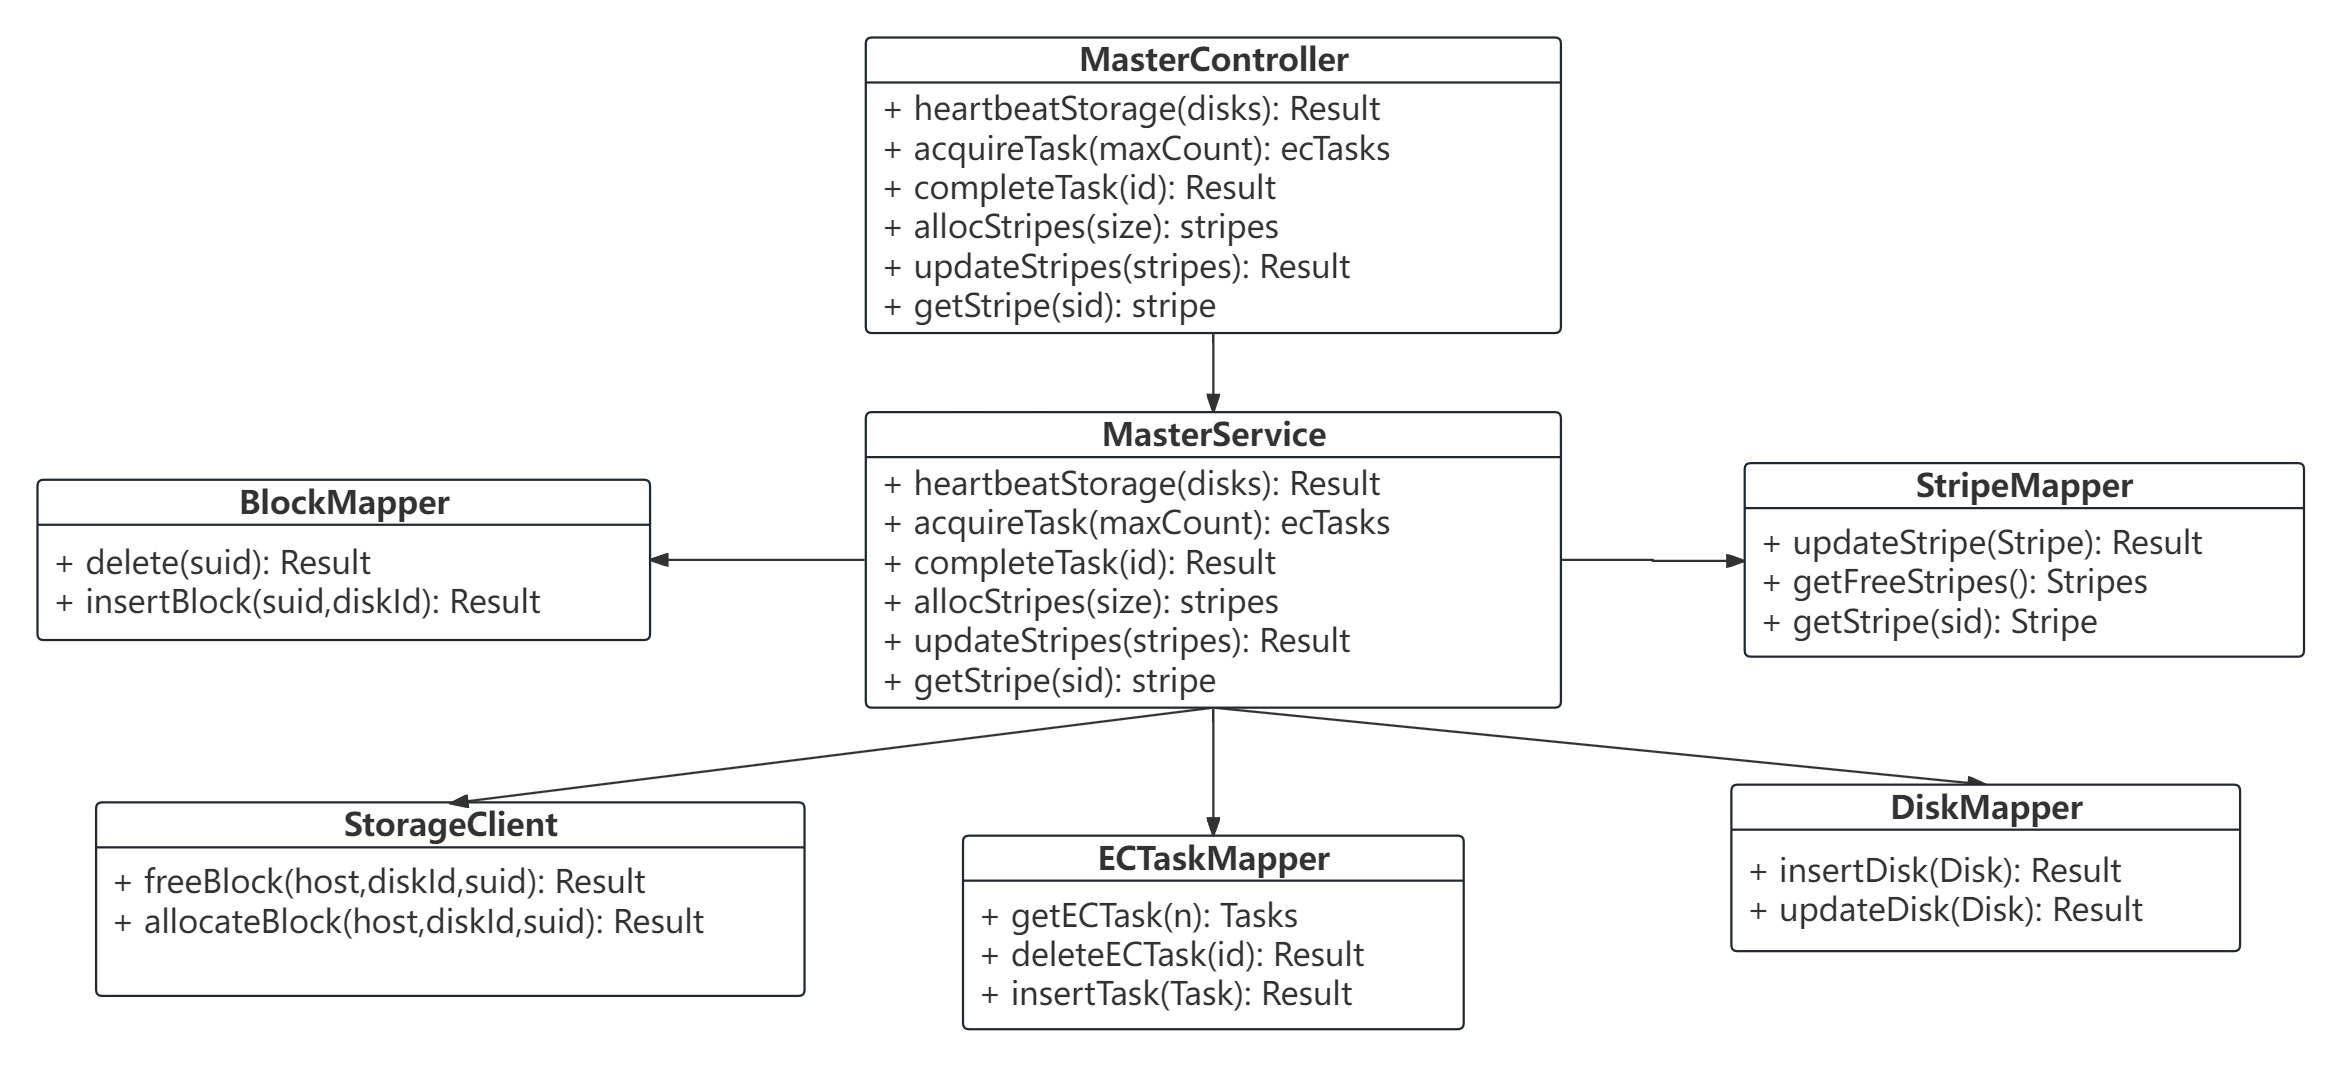
\includegraphics[width=1\textwidth]{master类图.jpg}
  \caption{master类图}
\end{figure}

以上介绍了master的类的组成,接下来将介绍master接口的实现细节。

1. heartbeatstorage接口

这个接口的作用是收集系统中磁盘信息,在master刚运行时,磁盘表是空的,master通过开放这个接口获取storage的心跳,从而得知storage下管理了多少磁盘和相关的磁盘信息。这个接口的请求体内需要有totalCount和availCount字段,它们和磁盘集合中的字段意义相同,分别代表磁盘内总块数和可用块数,请求体中无需提供host,host可以在HTTP请求中得到。

在接收请求后,MasterController会将请求转发给MasterService,MasterService会先将请求中没有diskId的数据取出来,这些磁盘是第一次在master中登记,MasterService会为它们分配diskId,在响应体内告知storage磁盘对应的diskId,并使用DiskMapper的insertDisk方法来保存这些新加入系统的磁盘信息;对于请求中标有diskId的数据,代表这些磁盘已经登记过,只需要使用DiskMapper的updateDisk方法来对磁盘信息做出更新即可。

2. EC任务相关接口

和EC任务相关的接口有两个,一个是woker获取任务接口,另一个是worker完成任务接口。其中worker获取任务接口比较容易实现,master在收到这个HTTP请求后用ECTaskMapper的getECTask方法在EC任务集合中寻找state为0的任务,然后根据worker给出的maxCount返回指定的任务即可。

worker完成任务接口是worker完成EC任务时为通知master所调用的接口,这个接口需要在请求体中给出已完成EC任务的任务id,这个接口主要流程如图5.2所示。

\begin{figure}[h]
  \centering
  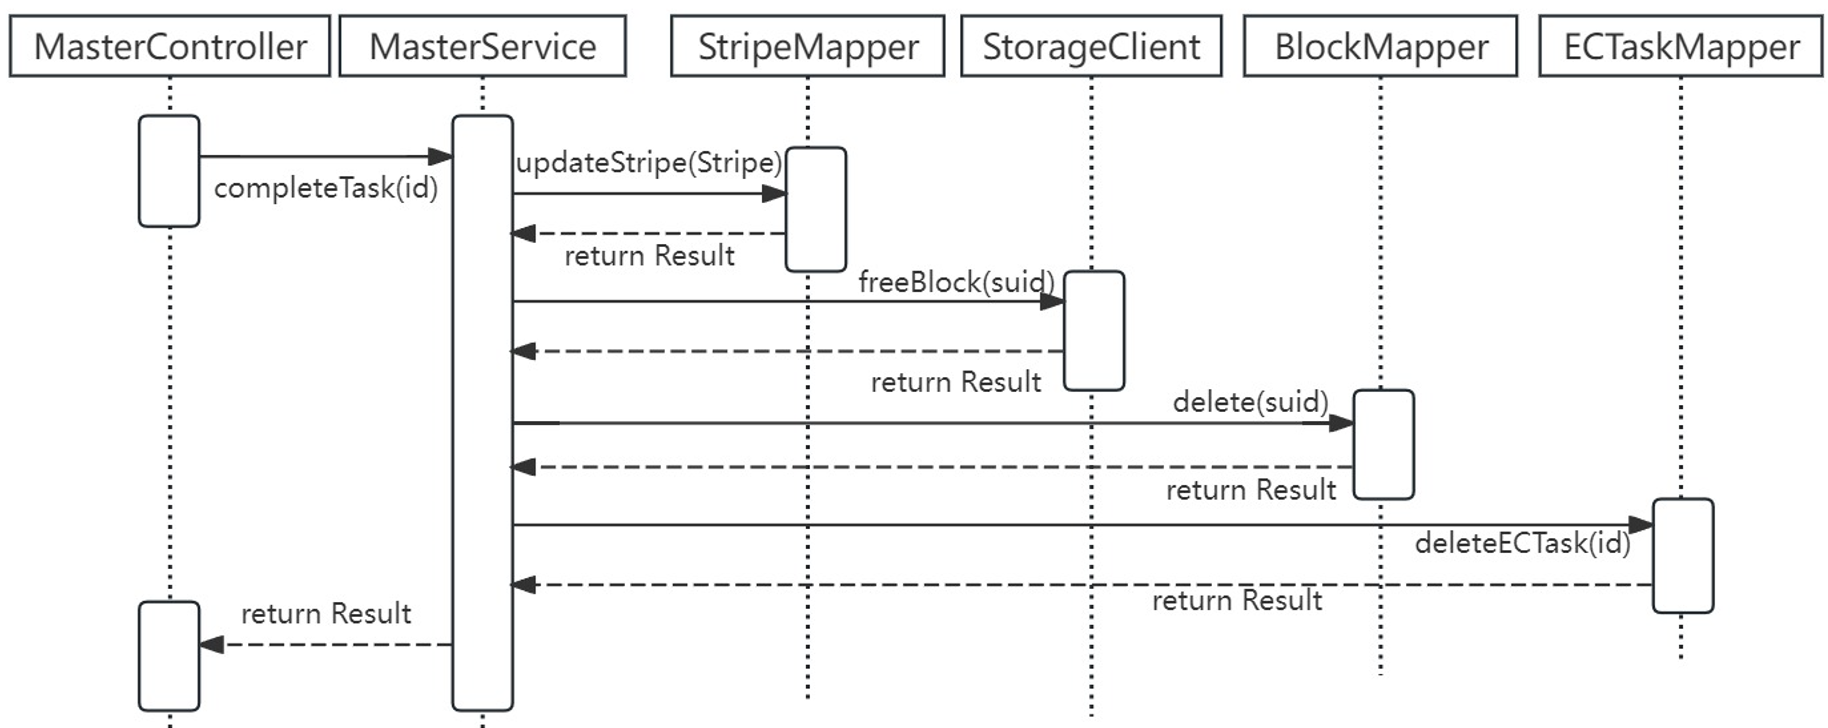
\includegraphics[width=1\textwidth]{worker完成任务时序图.png}
  \caption{worker完成任务时序图}
\end{figure}

master在收到这个请求后将会进行以下工作:用StripeMapper的updateStripe方法在条带集合中将已经完成EC的条带的state置为3;调用StorageClient的freeBlock方法将冗余块和条带进行解绑;用BlockMapper的delete方法在块集合中删除已EC条带中多余的块与磁盘的映射关系,最后,master还需要用ECTaskMapper的deleteECTask方法将EC任务集合中对应的任务删除。

3. 分配条带接口

当新文件需要写入到系统中时,需要为这个文件分配条带,这个接口的主要作用就是根据条带中块的分布规则建立新的条带,分配条带的大致流程如图5.3所示。

\begin{figure}[h]
  \centering
  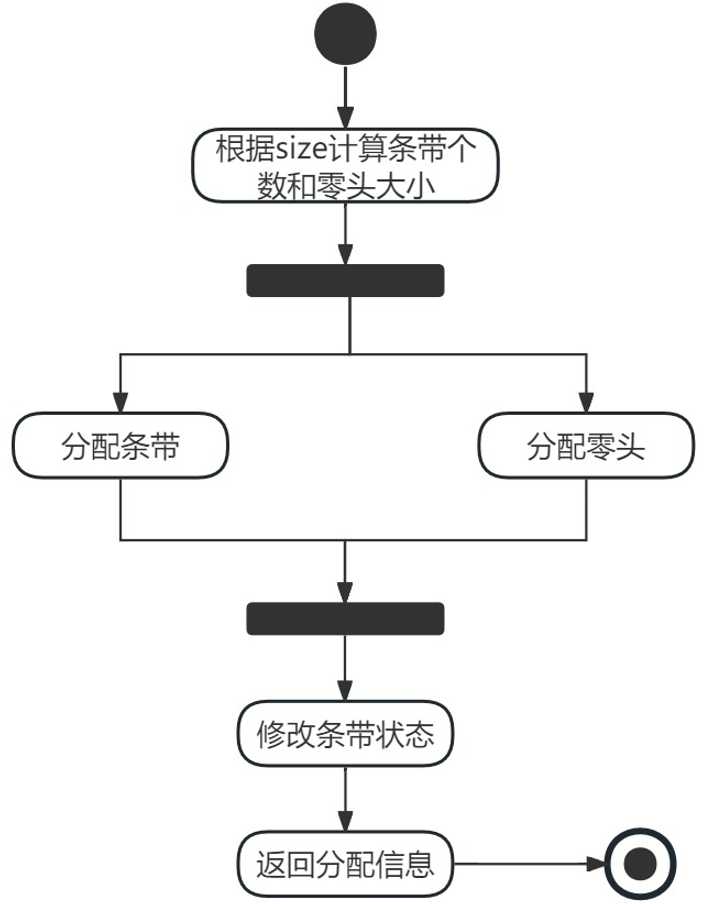
\includegraphics[width=0.5\textwidth]{分配条带详细活动图.png}
  \caption{分配条带活动图}
\end{figure}

首先需要根据接口的size参数除以条带的容量大小得到所需的条带个数和容量零头,然后会同时进行整个条带和零头的分配。对于整个条带的分配,需要根据块分配策略在不同的磁盘上使用空闲块将条带组合,这个过程中首先用BlockMapper的insertBlock方法将块分配到磁盘的信息记录下来,然后需要调用StorageClient的allocateBlock方法告知对应的storage磁盘上的块已经被使用;对于容量的零头,需要调用StripeMapper的getFreeStripes方法获取可以分配的条带,然后将可分配容量从小到大进行排序,依次与容量零头进行匹配,当找到第一个容量大于零头的条带则匹配成功,反之则为匹配失败,需要为这个零头建立一个新的条带。在所需的空间建立好之后,需要使用StripeMapper的updateStripe方法将这些条带的state改为1,代表它们不能再次被分配。最后master需要将分配的条带信息进行整理,将信息进行返回。

4. 条带相关接口

和条带相关的接口有两个,一个是获取条带信息的接口,另一个是更新条带信息的接口。获取条带信息的接口相对容易实现,在参数中获取所需要的条带id,然后使用StripeMapper的getStripe方法即可获得条带的信息,将此信息返回即可。

更新条带信息的接口主要是来处理条带状态问题的,在allocstripes接口分配条带之后,这些被分配的条带将会被锁定,不能再次被分配,只有获得条带使用权的服务调用updateStripes接口后才能解封,解封的过程将使用StripeMapper的updateStripe方法实现,解封后将条带的state置为0并将更新remainingCapacity。如果remainingCapacity为0,意味着这个条带已被写满,那么这个条带可以进行EC操作,将多余的副本删去。master将会用ECTaskMapper的insertTask方法向EC任务集合中插入一个EC任务,创建EC任务需要填写EC任务集合中的hosts字段和mode字段,hosts字段需要将条带中块的访问地址按照块的顺序放置到数组中。在这里填写这个字段的目的是聚焦worker的任务,使worker能专注于EC任务的执行,无需再次访问master去获取块的地址。

\subsection{storage实现}%5.4.2
storage的类图如图5.4所示,StorageController负责开启服务,监听其他服务的请求,StorageController收到请求后会将请求转发给StorageService。StorageService中借助DiskTool来读取和写入磁盘数据,DiskTool使用系统调用来读取本机上的磁盘信息。

\begin{figure}
  \centering
  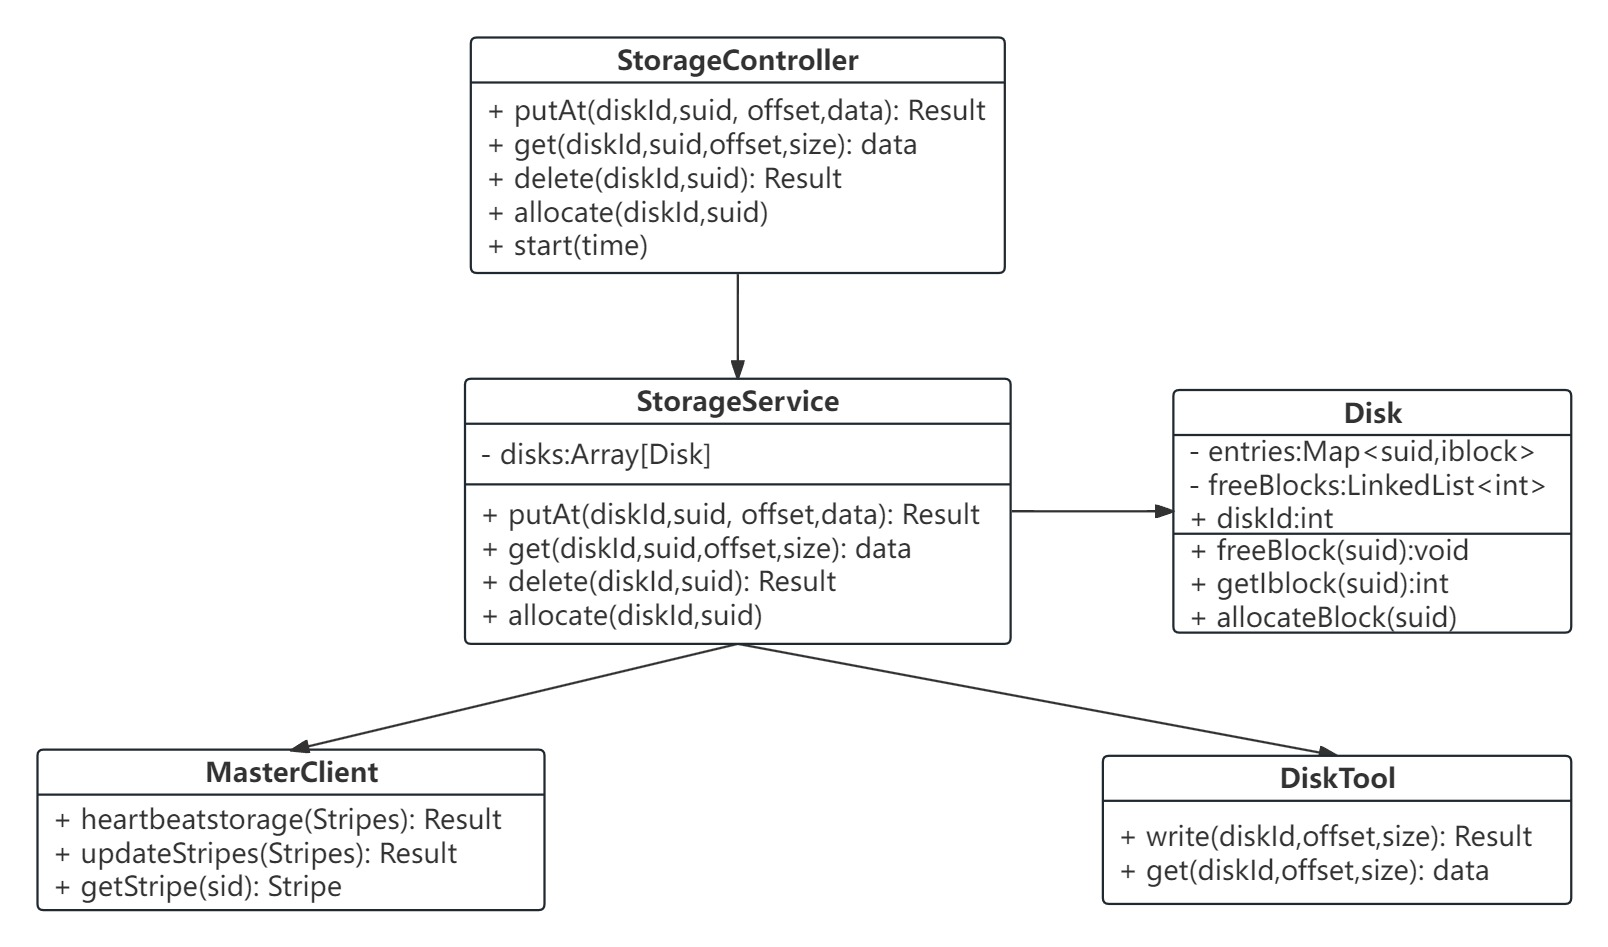
\includegraphics[width=1\textwidth]{storage类图.jpg}
  \caption{storage类图}
\end{figure}

在storage内部还需要一些数据结构来保存块和磁盘的相关信息,需要重点介绍Disk类。Disk内有两个数据结构,分别是entries和freeBlocks,entries是一个map,用于记录suid到iblock的映射,iblock指的是某个块在整个磁盘中是第几个块,保存iblock的目的是,读写磁盘的系统调用需要给出读取位置在磁盘中的偏移量,有了iblock就可以快速定位块的位置。freeBlocks是一个链表,这个链表记录了磁盘内部哪些块可以被分配,链表中每个节点也需要保存iblock的信息。Disk类对外提供了三个方法,freeBlock方法可以使已经被分配的块重新加入freeBlocks;getIblock可以根据suid获取这个块在磁盘中的偏移量;allocateBlock可以将某个空闲块分配给指定的suid。freeBlock方法和allocateBlock方法在修改内存中数据结构的同时,也会修改磁盘上的信息,进行数据块的分配和释放。

在storage启动时会调用start方法,这个方法的主要作用是给storage进行初始化,具体的执行流程如图5.5所示。storage先会将机器中所有的磁盘依次读取,检查它们的头信息区,如果发现没有初始化,则会先去获取磁盘的容量,计算出这块磁盘总共可容纳多少个块,将头信息区中的内容进行填写,然后读取磁盘的目录区,在storage的内存中为每块磁盘初始化Disk类,建立entries和freeBlocks这两个数据结构,最后将磁盘的信息以心跳的方式发送给master,在收到响应后,将新磁盘的id填入头信息区内。此后storage将每隔一段时间向master发送心跳,汇报机器内的磁盘信息。

\begin{figure}
  \centering
  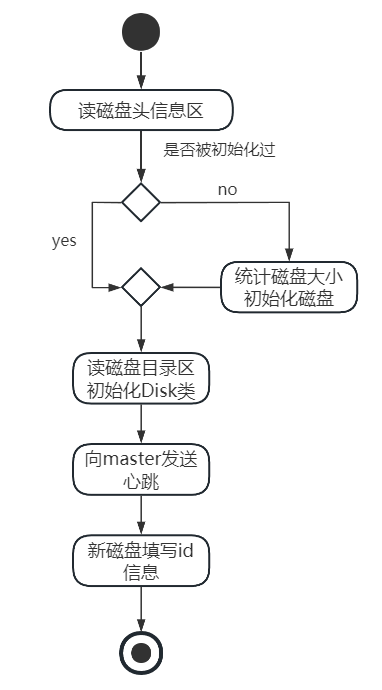
\includegraphics[width=0.45\textwidth]{start活动图.png}
  \caption{start活动图}
\end{figure}

以上介绍了storage的类的组成,接下来介绍接口的实现细节。

1. 上传数据接口

在上传数据的接口中提供了diskId,suid,offset和size这四个参数,通过diskId可以定位到对应的磁盘,定位到对应的磁盘后,storage可以根据suid用Disk类的getIblock方法从entries中查找记录,读取记录中iblock的值,利用接口参数中的offset和iblock值可以计算出所写区域的偏移量,然后调用DiskTool的write方法向磁盘内写入size大小的数据,同时更新BlockInfo中的DataLen和CRC32。

2. 下载数据接口

下载接口的实现和上传数据接口类似,首先用Disk类的getIblock方法从entries中查找记录,如果没有记录则返回错误,否则计算数据的偏移量调用DiskTool的read方法读取size大小的数据即可。

3. 删除块接口

和上述两个接口一样,首先要根据suid查找块记录,若没有记录则直接返回错误。若找到记录,将目录条目中的DeleteTime设置为当前时间并写入磁盘目录区。需要注意的是此时不能将此块进行释放,因为这个块仍然属于条带内的一部分,依然有可能继续向这个块中写入数据。

4. 分配块接口

当master新建一个条带时,需要将空闲的块当做条带的一部分,此时master会调用这个接口将某个磁盘上的一个空闲块分配给suid对应的块。storage接到这个请求后,需要利用Disk类中的allocateBlock方法将空闲块从空闲链表中取下,然后allocateBlock方法会将这个块和suid绑定加入到entries中去。同时,allocateBlock方法也会将对应块的头信息区和blockInfo填入接口参数的suid。

5. 释放块接口

当条带被回收或者EC任务进行完毕后,一些块不再隶属于条带,此时需要调用这个接口将这些块进行释放。storage接到这个请求后会调用Disk类中的freeBlock方法来释放块,freeBlock方法先到entries中找到这个suid对应的记录,然后将这个块的iblock信息加入到freeBlocks链表中,再将这条记录从entries中删除。同时,freeBlock方法也会将对应块的头信息区和blockInfo中的suid信息删除。

为了保证可扩展性,storage服务支持扩容,既可以以磁盘为单位进行扩容,也可以以storage为单位进行扩容。在以磁盘为单位进行扩容时,需要在storage服务所在的主机上增加磁盘,然后重启storage服务,storage重启后会检测到新磁盘的存在,storage会将新磁盘的信息发送给master,获得diskId后对磁盘进行初始化即可使用。以storage为单位进行扩容更加容易,只需在一台新主机上启动storage服务,然后将master的访问地址进行配置,storage会将本机的信息汇报给master,此后这台storage即可正常使用。

\subsection{worker实现}%5.4.4
本部分阐述worker的实现细节,在概要设计中阐述了worker的主要执行步骤,本部分重点介绍EC任务的执行细节。

worker的类图如图\ref{worker类图}所示。其中WorkerService是服务的主进程,它在启动时会执行start方法,这个方法有time和n两个参数,代表多长时间去master那里获取任务和一次获取多少,这两个量可以根据数据的写入情况进行配置,MasterClient和StorageClient分别是和master服务和storage服务通信的工具,封装了用接口访问它们的流程,EcCalculator是用来计算EC校验码的,通过encode方法可以算出对应数据的EC校验码。

\begin{figure}
  \centering
  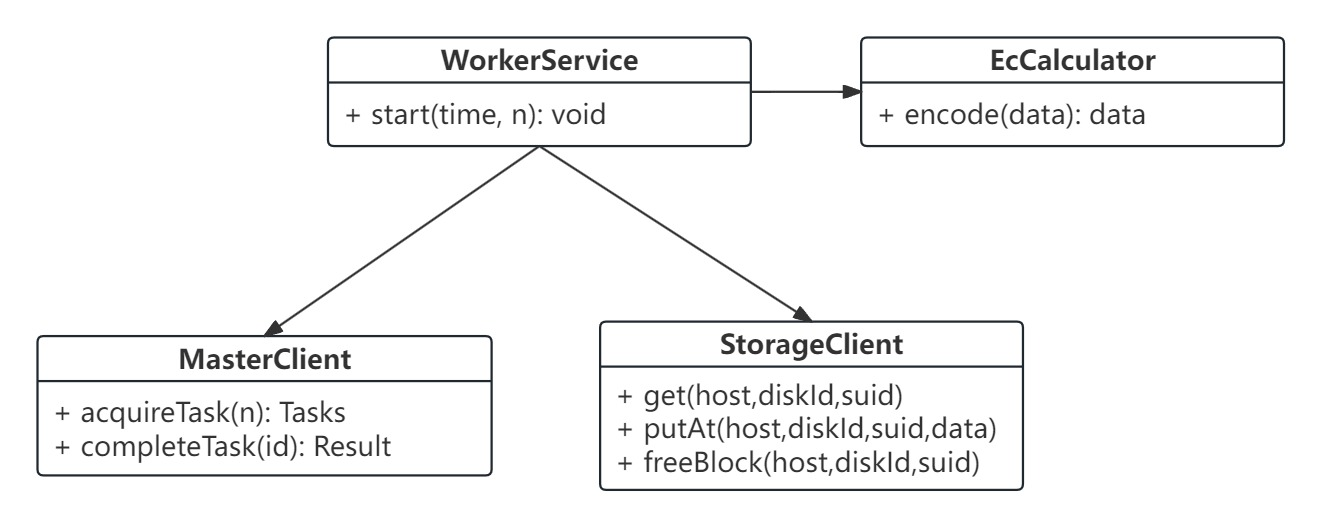
\includegraphics[width=0.8\textwidth]{worker类图.jpg}
  \caption{worker类图}
  \label{worker类图}
\end{figure}

图\ref{worker时序图}是worker完整执行一次任务的时序图。首先调用acquireTask方法从master获取EC任务,获取到的EC任务中有mode字段,根据mode可以得知条带的块分配模式,从而得知一个副本有几个块,一共需要生成多少校验块。通过hosts和disks这两个字段,可以得知访问相关数据块的具体地址信息。根据得到的信息,worker会调用get方法从storage那里读取需要执行EC任务的条带内数据,worker会并发地调用storage的接口,获取每个块的数据。在得到某个副本的全部数据后,将调用encode方法在本地进行EC计算,得出校验块的数据。然后用putAt方法调用storage的接口将得到的校验块的内容写入磁盘中。最后将会调用master的completetask接口,告知master此次EC任务已经执行完成。

\begin{figure}
  \centering
  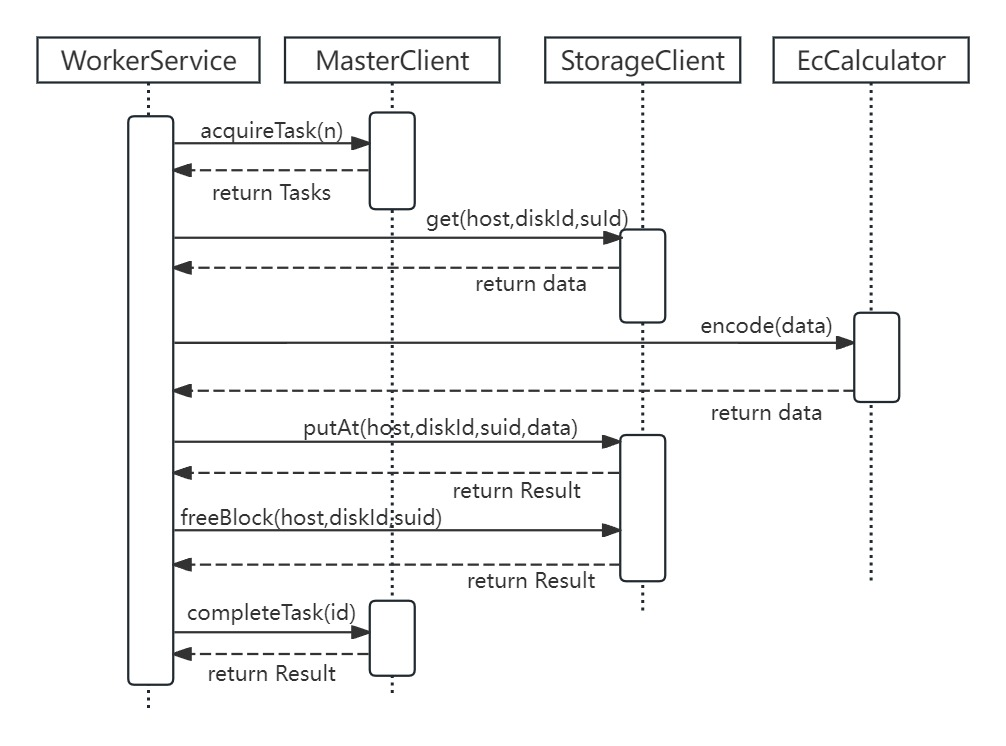
\includegraphics[width=0.75\textwidth]{worker时序图.jpg}
  \caption{worker时序图}
  \label{worker时序图}
\end{figure}

可以注意到上述过程中实现了多副本存储到纠删码存储的转换,但是无需进行额外的数据迁移,只需要异步地调用接口将数据删除即可,这是基于条带的文件分配模式的好处。

\subsection{msf实现}%5.4.3
msf是一个代码库,上层的功能模块可以引用这个代码库,调用msf提供的方法来完成数据操作,msf可以被视为对象数据存储模块的客户端,它为其他模块屏蔽了模块内部的细节,减轻系统的耦合。

\begin{figure}
  \centering
  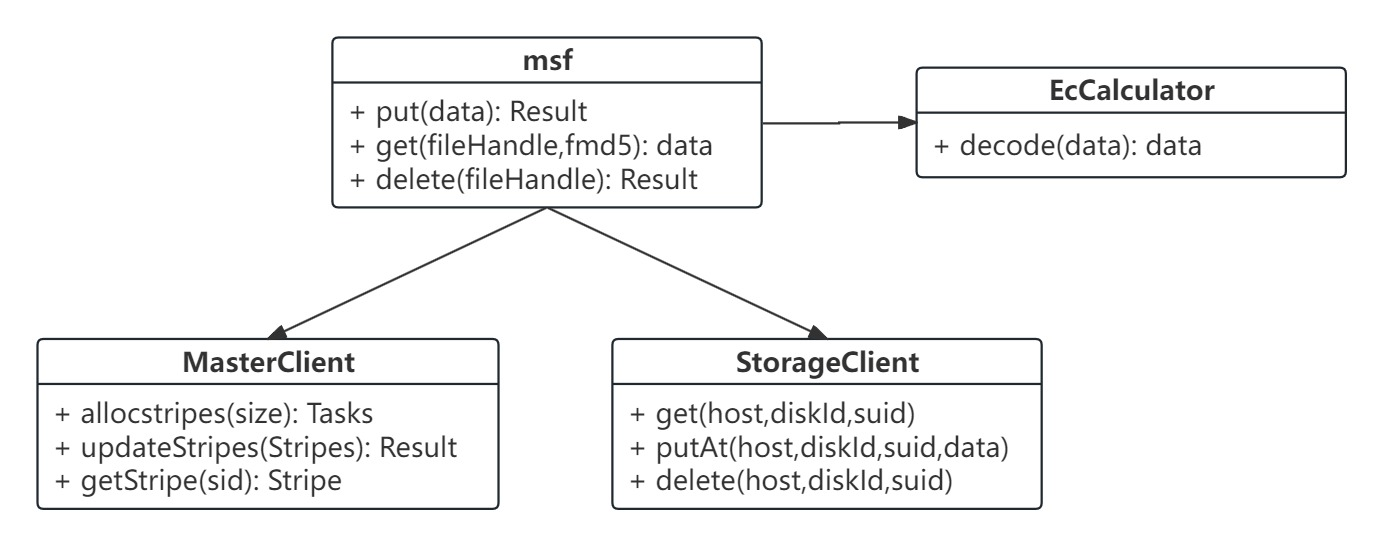
\includegraphics[width=0.8\textwidth]{msf类图.jpg}
  \caption{msf类图}
  \label{msf类图}
\end{figure}

msf的类图如图\ref{msf类图}所示,接下来主要阐述msf中的方法的实现细节。内部需要持有两个关键的对象,一个是MasterClient另一个是StorageClient,持有它们的作用是为了与master和storage进行交互。msf提供的三个方法都需要和它们进行交互。除此之外,msf还需要EcCalculator的支持,当需要进行纠删码解码的时候需要它将数据进行恢复。接下来将详细介绍每个方法在实现时是如何与其他服务进行交互的。

1. put方法

\begin{figure}[h]
  \centering
  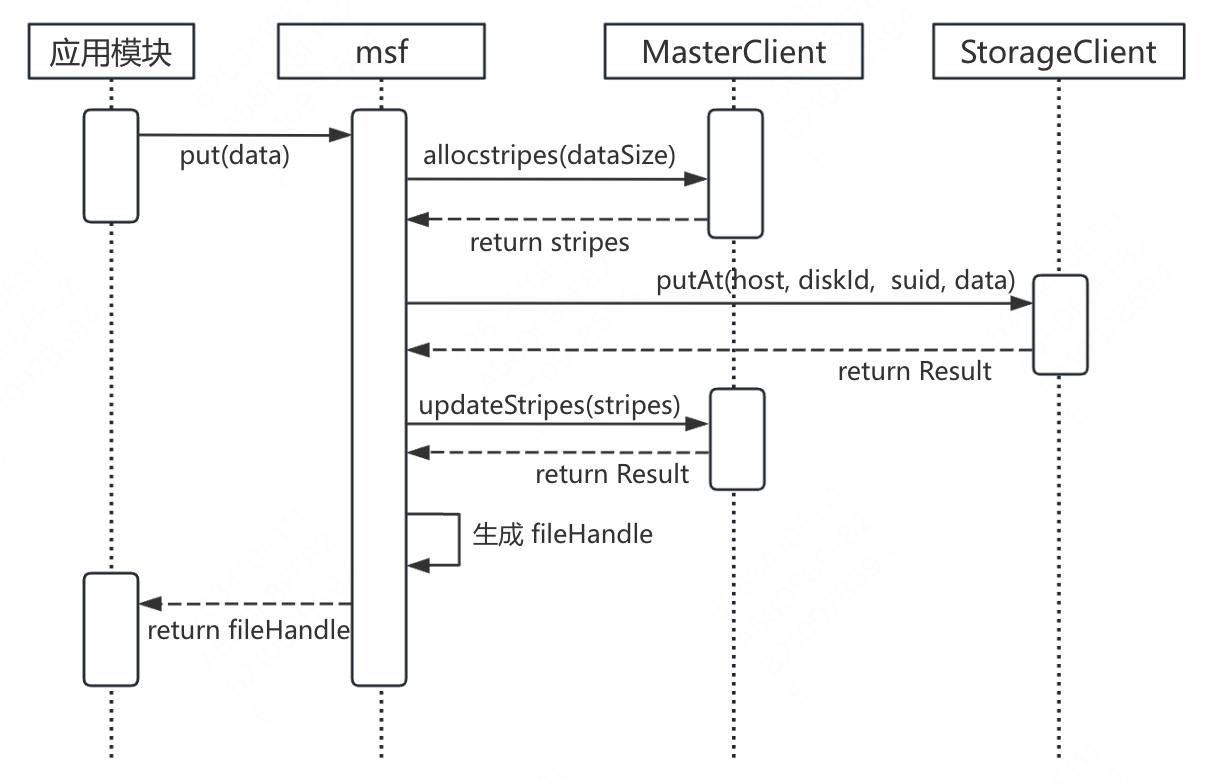
\includegraphics[width=0.7\textwidth]{put时序图.png}
  \caption{put方法时序图}
  \label{put方法时序图}
\end{figure}

put方法的执行过程如图\ref{put方法时序图}所示。put方法需要提供数据内容,msf由此会得到写入的数据的大小,msf会首先用MasterClient的allocstripes方法来调用master的allocstripes接口,根据给出的数据大小去申请条带,master会将分配的条带和块的相关信息一并返回。随后msf会调用StorageClient的putat方法,将数据写到对应的块中,写入不同的块可以并发执行。在数据都上传完毕后,msf会首先调用MasterClient的updateStripes方法来通知master申请的条带已经写入完毕,然后msf会根据返回的条带信息生成对应的fileHandle,再将生成的fileHandle进行返回。

2. get方法

\begin{figure}[h]
  \centering
  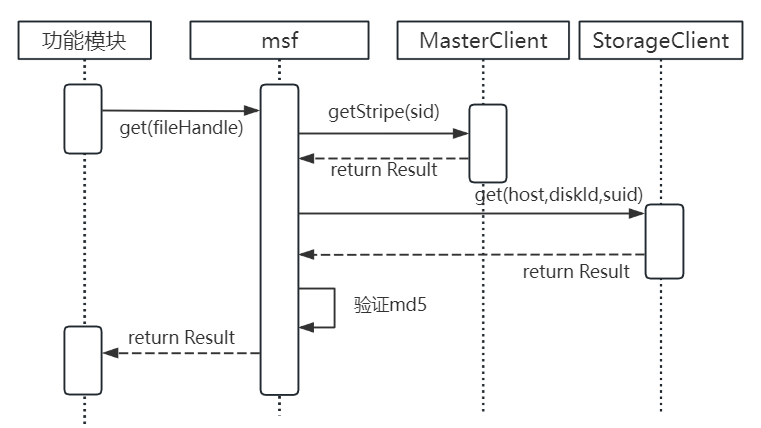
\includegraphics[width=0.7\textwidth]{get时序图.png}
  \caption{get方法时序图}
  \label{get方法时序图}
\end{figure}

get方法用于上层服务从存储模块下载数据,这个方法的执行过程如图\ref{get方法时序图}所示。调用这个方法需要提供fileHandle,msf在拿到参数中的fileHandle之后需要调用反序列化方法,将二进制信息反序列化为fileHandle。得到fileHandle后,利用fileHandle中的StripeIds字段调用MasterClient的getStripe方法获取文件所在条带的块信息和磁盘信息。得到这些信息后,msf会根据已知的块信息调用StorageClient的get方法,由于条带内部的块不会分布在同一台机器上,所以读取块数据的操作会并发执行。如果在调用接口的过程中出现调用超时或者下载后数据的md5与参数中的md5不相同的情况,则需要根据当前条带的状态来访问冗余信息:如果是多副本状态,那么需要访问与故障块互为冗余的块数据;如果是纠删码状态,则需要读取一定数量的校验块和数据块,用EcCalculator中的decode方法将故障数据进行计算恢复。在所有数据读取完毕后,msf会将读取的数据进行整理统计,将文件数据data进行返回。

3. delete方法

delete方法需要上层服务提供fileHandle,和get方法一样,需要先得到fileHandle再调用MasterClient的getStripe方法获取文件所在条带的块信息和磁盘信息。接下来msf会根据得到的块信息调用StorageClient的delete方法将条带内的块数据进行删除。最后调用MasterClient的updateStripes方法来告知master条带的变动情况。

\section{功能模块实现}%5.4
在上一节中介绍了对象数据存储模块的具体实现方案,这一小节来介绍功能模块的实现方案。

\subsection{用户数据管理模块实现}
用户数据管理模块向用户提供管理用户数据的功能,具体包括创建用户、修改用户信息和查看用户信息这三个功能。这个模块的类图如图\ref{用户数据管理模块类图}所示。

\begin{figure}
  \centering
  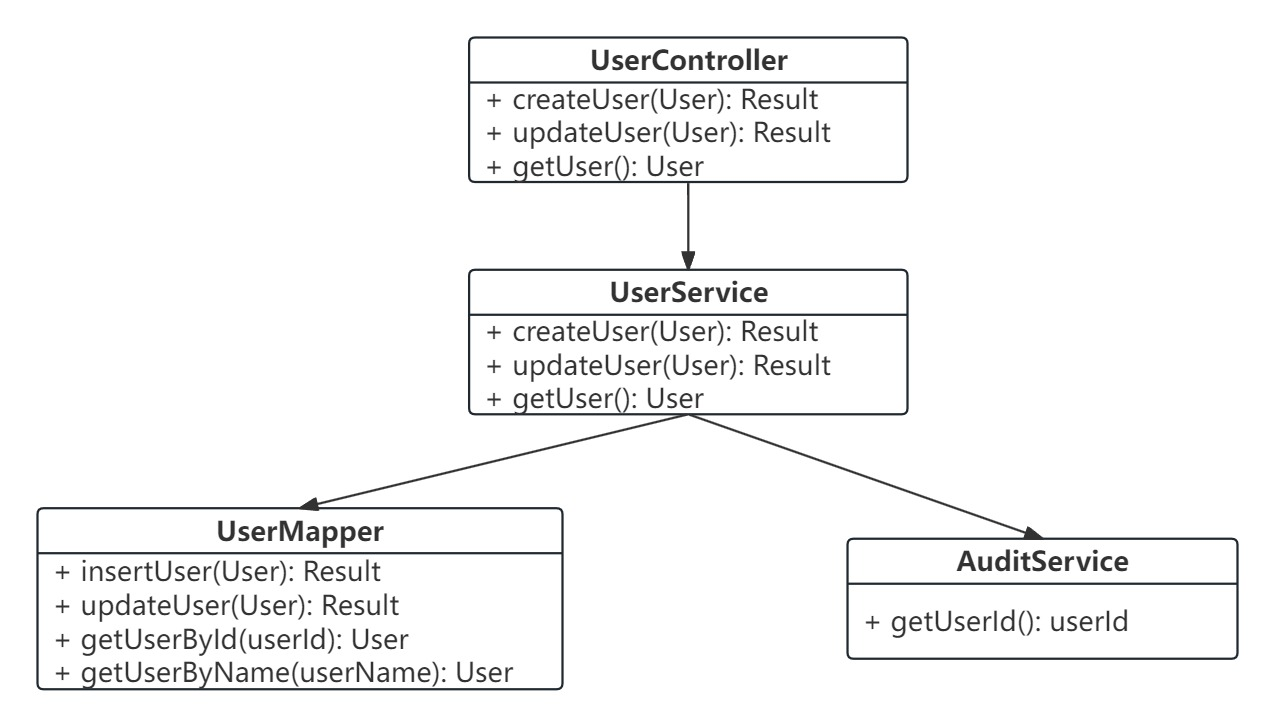
\includegraphics[width=0.7\textwidth]{用户数据管理类图.jpg}
  \caption{用户数据管理模块类图}
  \label{用户数据管理模块类图}
\end{figure}

UserController是用户数据管理模块的入口,负责接收用户的请求。UserService负责处理具体的功能逻辑。UserMapper是和元数据数据库交互的接口,UserMapper和MongoDB建立连接,保存用户数据或查找用户数据。AuditService是来管理鉴权信息的类,在用户鉴权通过后,可以通过getUserId方法来获取当前用户的uid,以进行下一步的操作。

\begin{figure}
  \centering
  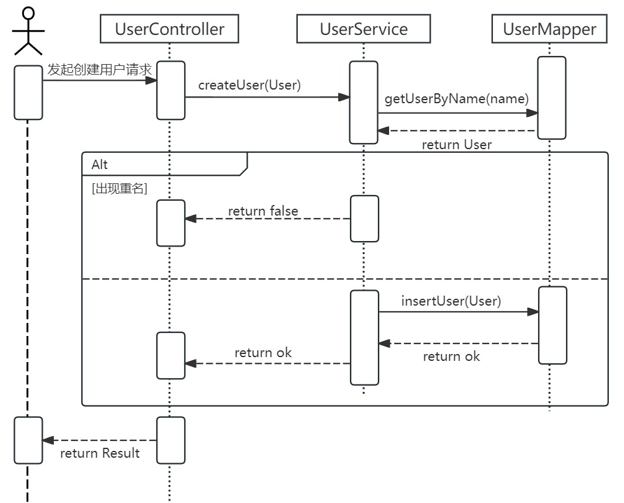
\includegraphics[width=0.68\textwidth]{创建用户时序图.png}
  \caption{创建用户时序图}
  \label{创建用户时序图}
\end{figure}

创建用户的时序图如图\ref{创建用户时序图}所示。创建用户流程始于客户端通过UserController发起的创建用户请求,该请求携带了用户的基本信息,UserController会将请求转发给UserService,UserService在收到请求后会先调用UserMapper中的getUserByName方法来验证是否出现了重名的情况,如果有的话则直接返回错误的结果,反之则调用UserMapper中的insertUser方法将用户数据保存至元数据数据库中,实现信息的持久化。

修改用户信息的时序图如图\ref{修改用户信息时序图}所示。UserController接收到用户的修改信息的请求后,会调用updateUser方法将信息传递给UserService,UserService会先调用AuditService中的getUserId方法来验证用户是否已经通过鉴权,如果没有则直接返回错误,反之则会调用UserMapper中的updateUser方法,在元数据数据库中修改这位用户的信息。

\begin{figure}
  \centering
  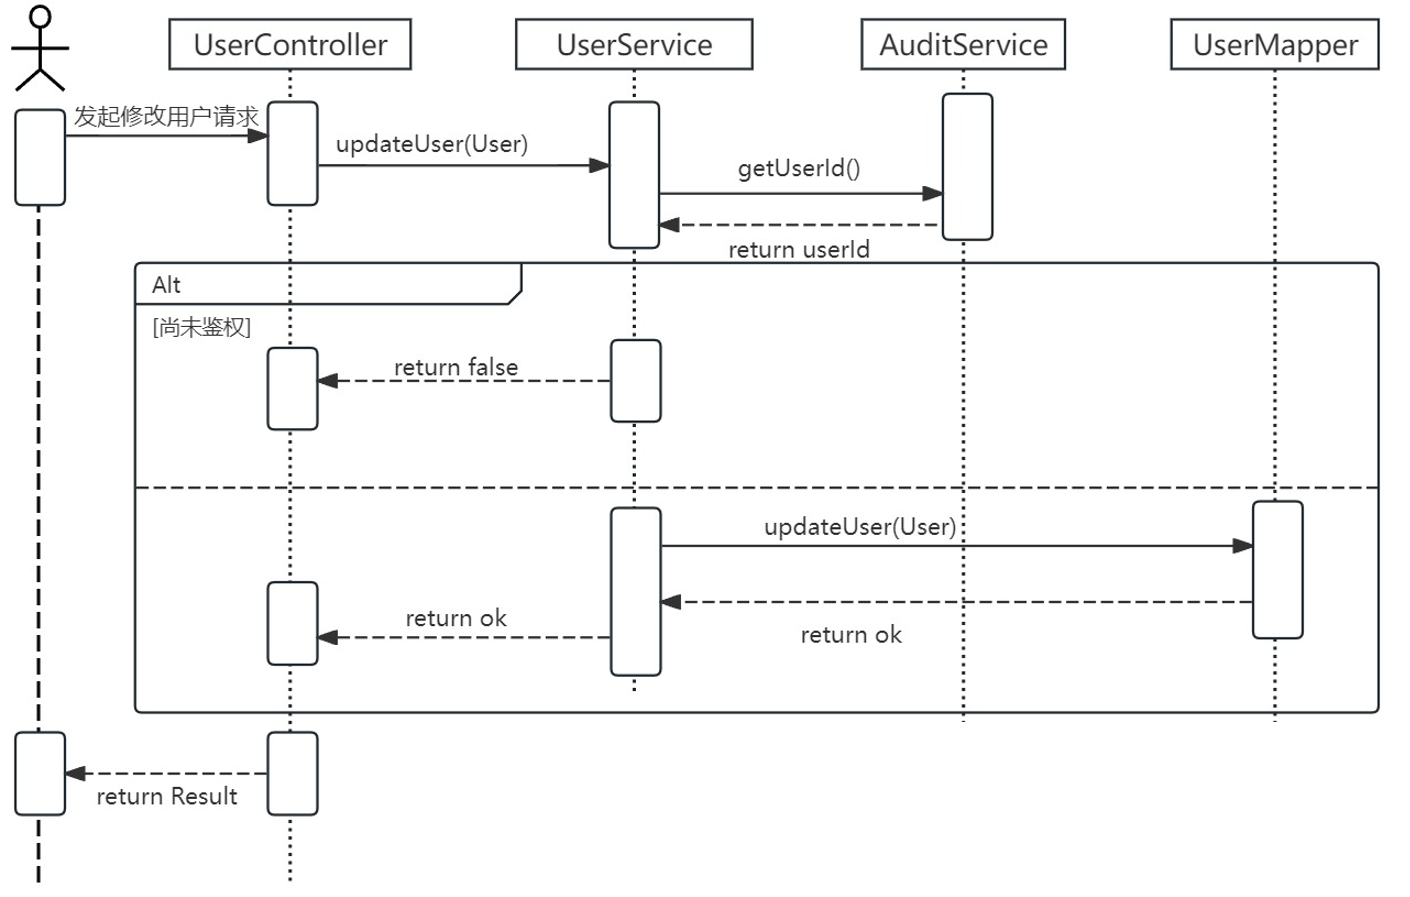
\includegraphics[width=0.8\textwidth]{修改用户时序图.png}
  \caption{修改用户信息时序图}
  \label{修改用户信息时序图}
\end{figure}

查看用户的工作流程与图\ref{修改用户信息时序图}中的流程类似,只需要将UserController中执行的方法变为getUser,同时在鉴权通过的情况下调用UserMapper中的getUserById方法来从元数据数据库中获取用户信息。

\subsection{桶数据管理模块实现}

桶数据管理模块向用户提供管理桶数据的功能,具体包括创建桶、删除桶、修改桶信息和查看桶信息这四个功能。这个模块的类图如图\ref{桶数据管理模块类图}所示。

桶数据管理模块中的BucketController和BucketService用户数据管理模块的类图结构类似,是用来接收请求和实际执行业务操作的类。BucketService引入AuditService的原因是为了获取用户的uid,便于模块提供查看创建的全部桶的功能,BucketMapper中提供了getBucketByUid方法来支持这项功能。为了支持删除桶操作,BucketService引入了msf和FileinfoMapper来删除文件的元数据和实际数据。

\begin{figure}
  \centering
  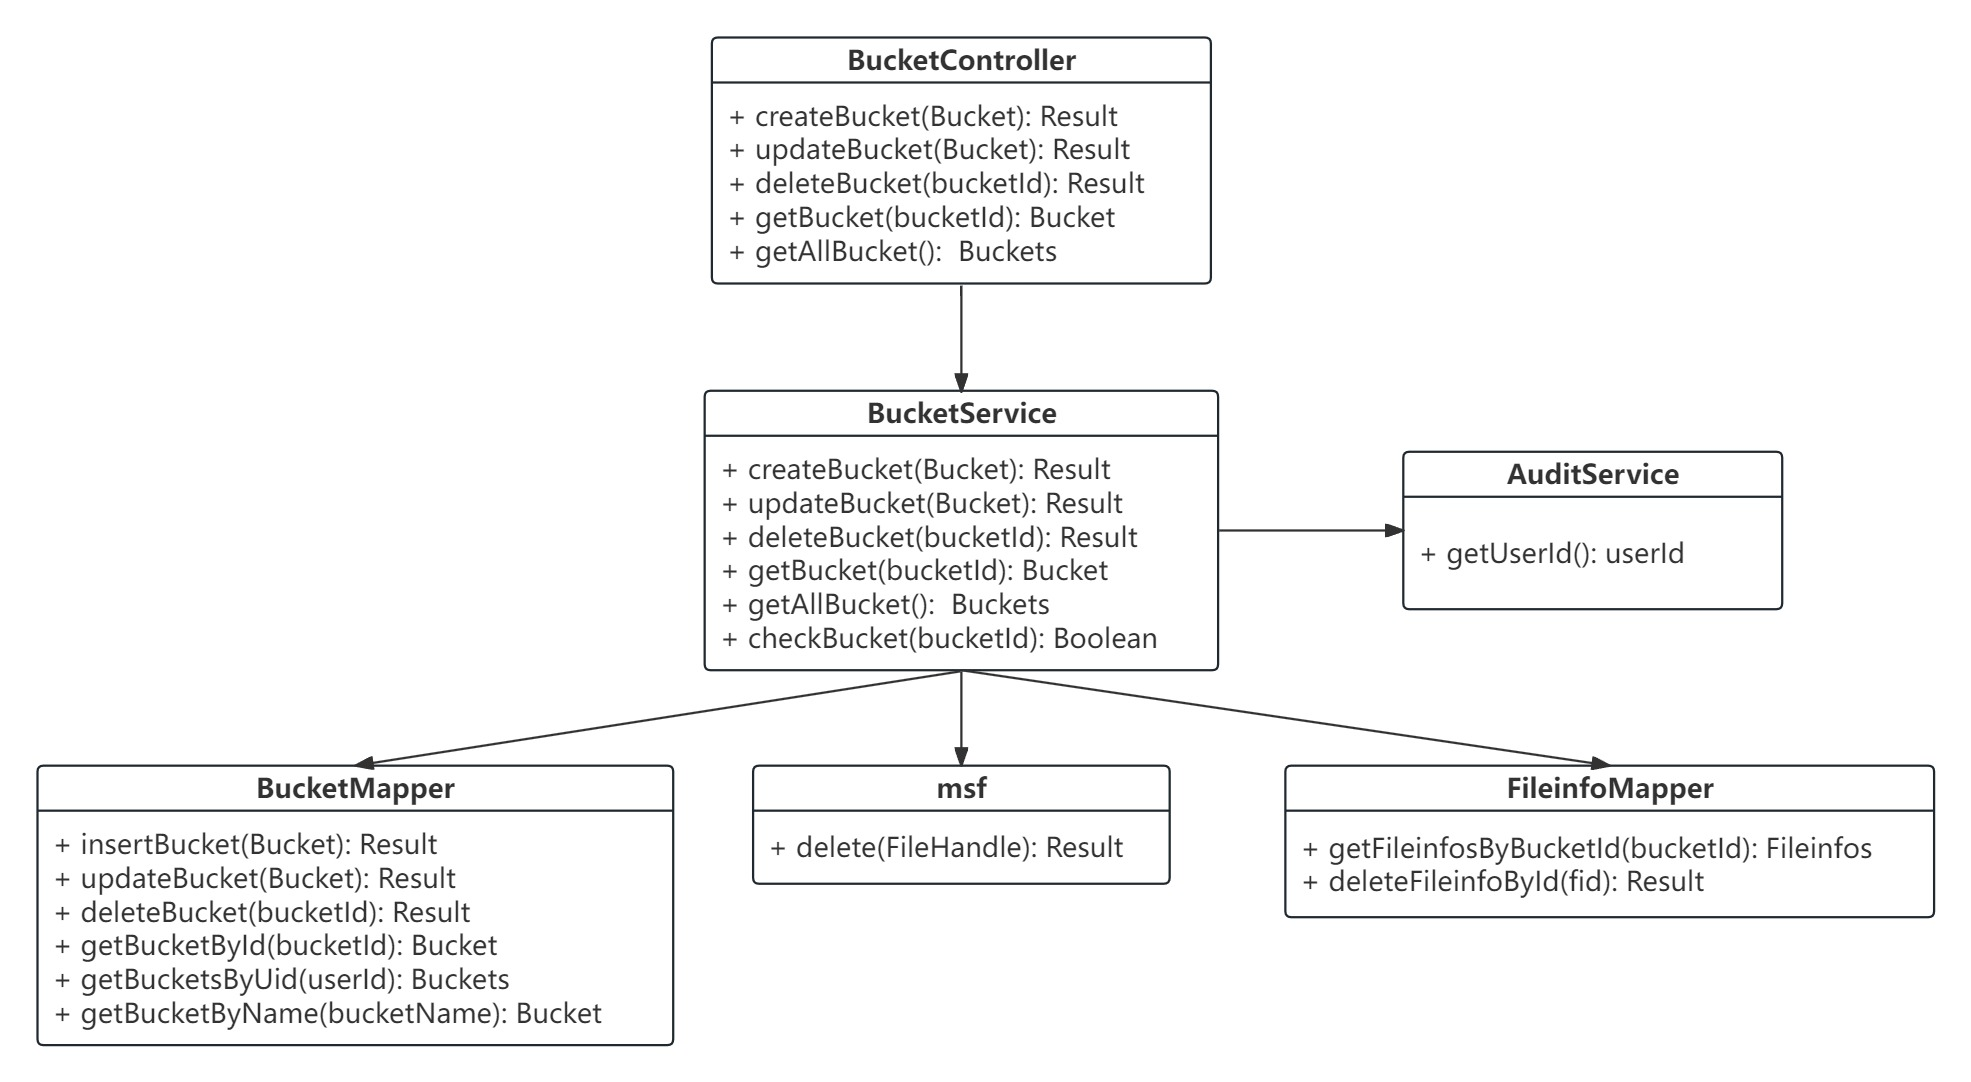
\includegraphics[width=0.9\textwidth]{桶数据管理类图.jpg}
  \caption{桶数据管理模块类图}
  \label{桶数据管理模块类图}
\end{figure}

在介绍操作的具体实现之前,首先需要介绍BucketService中的checkBucket方法,它的作用是来检查一个桶是否是由请求用户创建的,由于这个操作在多个方法中都需要使用,为了代码能够更好地进行复用,需要将这些操作整合为一个方法。这个操作的具体流程是,首先调用BucketMapper的getBucketById方法验证桶是否存在,然后调用AuditService的getUserId方法来获取用户的uid,通过判断uid和桶的uid属性是否相同来确定桶是否由请求用户创建。

\begin{figure}
  \centering
  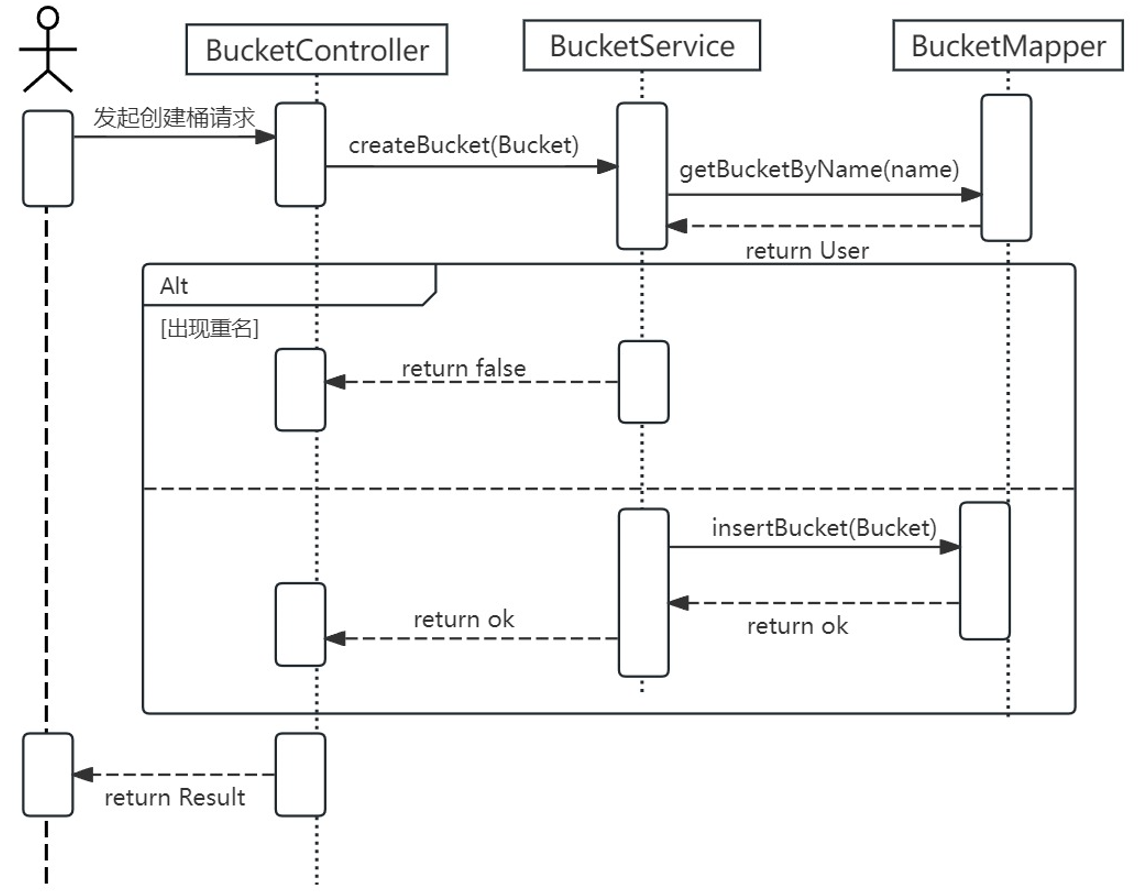
\includegraphics[width=0.7\textwidth]{创建桶时序图.png}
  \caption{创建桶时序图}
  \label{创建桶时序图}
\end{figure}

创建桶的时序图如图\ref{创建桶时序图}所示。BucketController在接收到请求后将请求转发给BucketService进行处理,BucketService首先会调用BucketMapper的getBucketByName方法来验证是否出现重名的桶,如果出现则直接返回错误,反之则会调用insertBucket方法将桶的相关信息保存到元数据数据库中并返回成功。

\begin{figure}
  \centering
  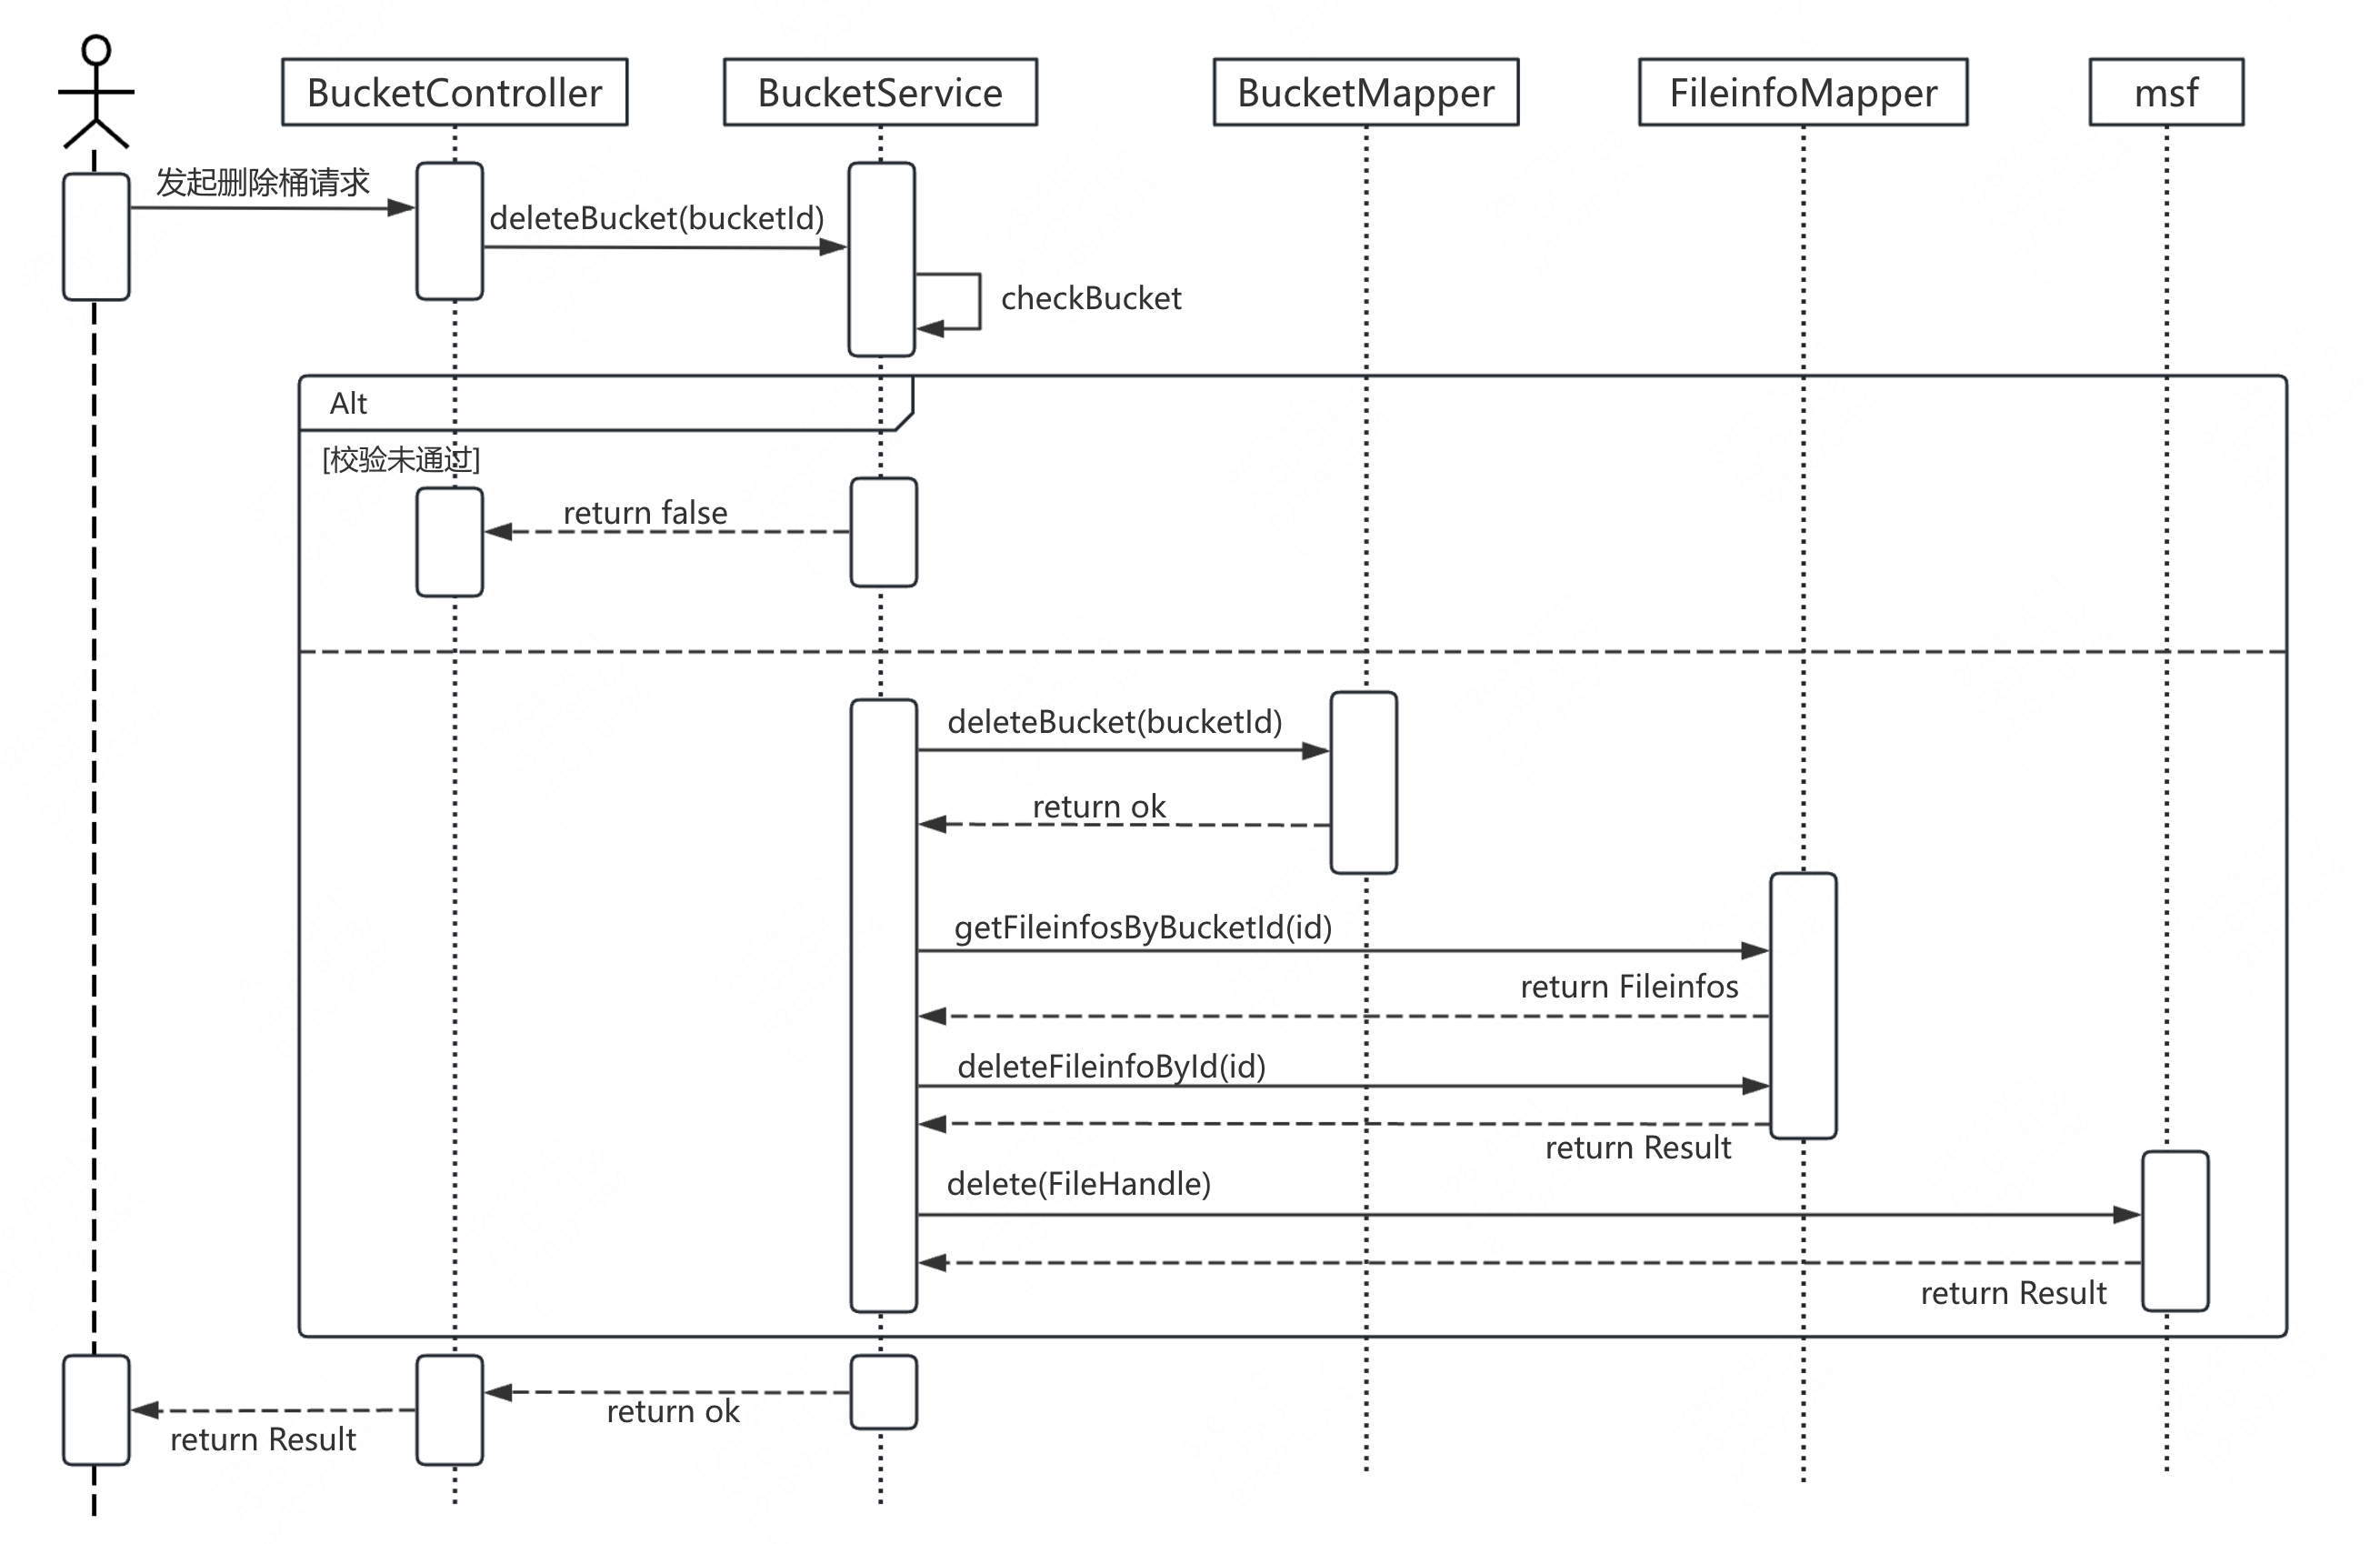
\includegraphics[width=0.9\textwidth]{桶删除时序图.png}
  \caption{删除桶时序图}
  \label{删除桶时序图}
\end{figure}

删除桶的时序图如图\ref{删除桶时序图}所示。BucketController在接收到请求后将请求转发给BucketService进行处理,BucketService首先会调用checkBucket方法来验证桶是否由自己创建且存在,验证成功后需要对桶内的数据进行删除,首先需要调用BucketMapper的deleteBucket方法将桶删除,然后会将桶内的文件删除,先调用FileinfoMapper的getFileinfosByBucketId方法来获取桶内所有的文件信息,然后依次调用FileinfoMapper的deleteFileinfoById和msf的delete方法将文件的元数据和实际数据进行删除。

\begin{figure}
  \centering
  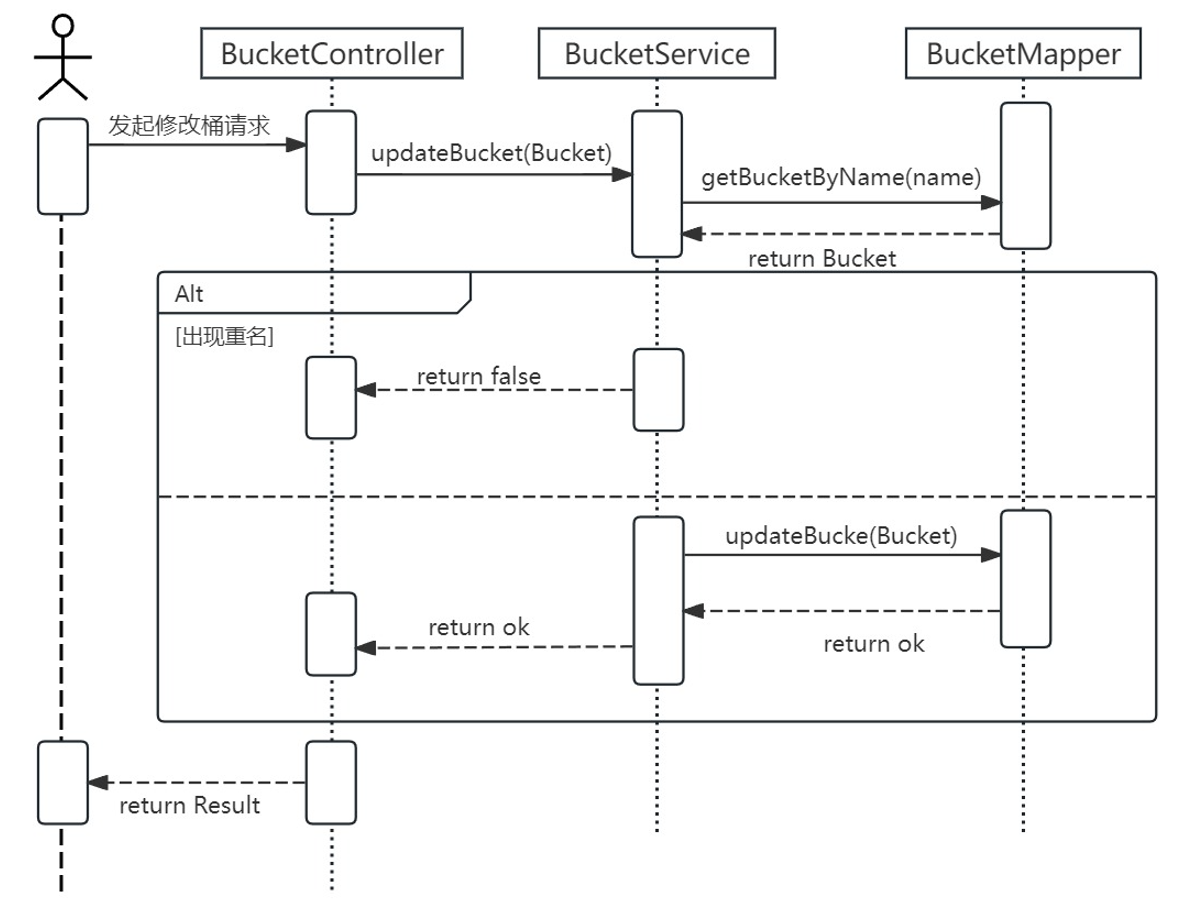
\includegraphics[width=0.75\textwidth]{修改桶时序图.png}
  \caption{修改桶信息时序图}
  \label{修改桶信息时序图}
\end{figure}

修改桶信息的时序图如图\ref{修改桶信息时序图}所示。开始的流程和删除桶的操作类似,都是将请求转发然后验证桶是否由自己创建,然后BucketService会调用BucketMapper的getBucketByName方法来验证修改后桶是否会重名,如果不会重名则会调用BucketMapper的updateBucket方法来更新桶信息。

查看桶数据的实现较为简单,在调用checkBucket方法验证通过后只需调用BucketMapper的getBucketById方法来获取桶信息。如果需要查看创建的全部桶信息,则需要先调用AuditService的getUserId方法来获取用户的uid,然后调用BucketMapper的getBucketsByUid方法来获取所需的信息。

\subsection{文件管理模块实现} 

\begin{figure}
  \centering
  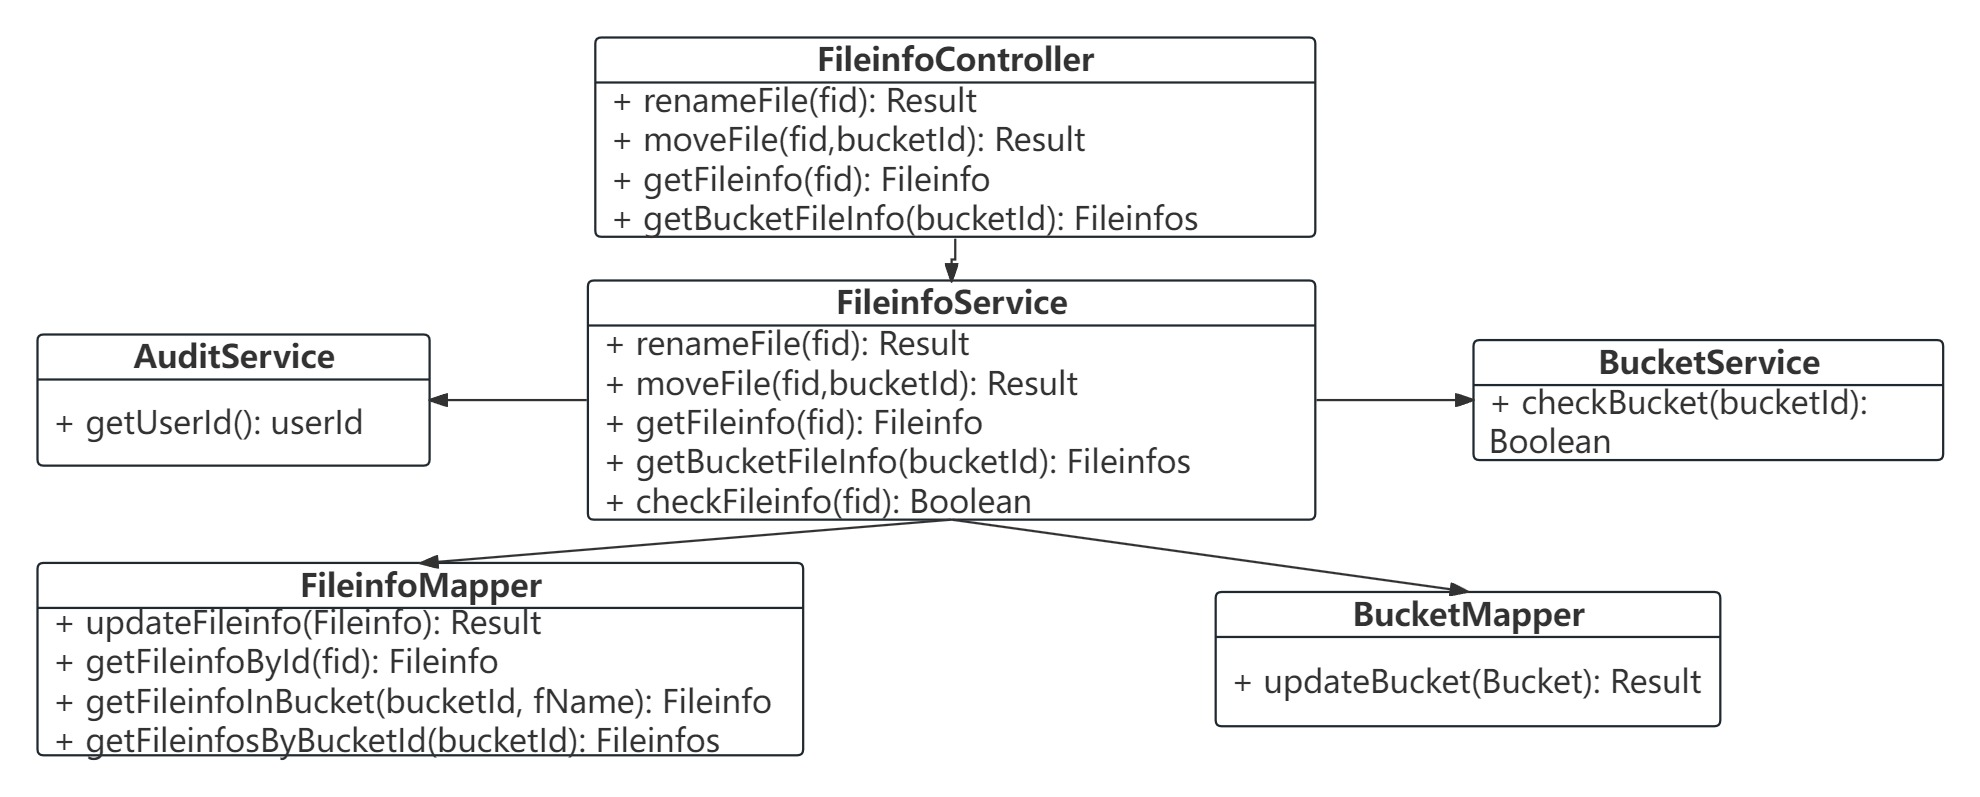
\includegraphics[width=1\textwidth]{文件管理类图.jpg}
  \caption{文件管理模块类图}
  \label{文件管理模块类图}
\end{figure}

文件管理模块向用户提供管理文件的功能,具体包括重命名文件、移动文件和查看文件信息这三个功能。这个模块的类图如图\ref{文件管理模块类图}所示。文件管理模块中值得介绍的是FileinfoService的checkFileinfo方法,它和BucketService的checkBucket方法类似,都是用来检测合法性的,在这里checkFileinfo用来检测文件是否存在且由自己创建,执行方法是先调用getFileinfoById方法检查文件是否存在,然后再判断文件中的uid属性和当前用户的uid是否相同,当前用户的uid可通过AuditService的getUserId方法获取。

重命名文件操作完整工作情况时的时序图如图\ref{重命名文件时序图}所示。FileinfoController将请求分发给后,FileinfoService会先调用checkFileinfo方法检测文件是否存在且由自己创建,如果检测通过则会用FileinfoMapper的getFileinfoInBucket方法来验证是否会出现重名的情况,如果不出现的话会调用updateFileinfo将文件进行重命名。\newline \newline \newline 

\begin{figure}
  \centering
  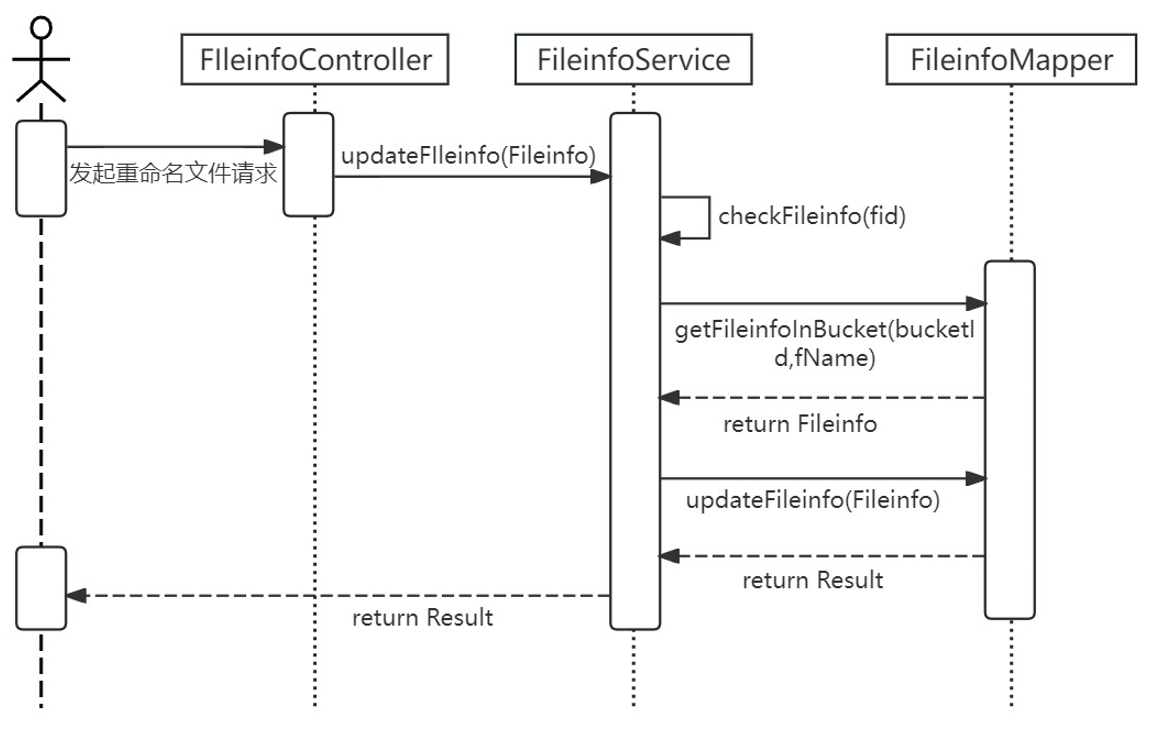
\includegraphics[width=0.8\textwidth]{重命名文件时序图.png}
  \caption{重命名文件时序图}
  \label{重命名文件时序图}
\end{figure}

移动文件操作完整工作情况时的时序图如图\ref{移动文件时序图}所示。和重命名文件一样,模块会先检测文件是否存在且由自己创建,如果检测通过还需要用checkBucket检测目标桶是否存在且由自己创建,如果检测通过,需要进一步用FileinfoMapper的getFileinfoInBucket方法检查移动会是否出现重名文件,如果不会出现则调用updateFileinfo将文件移动至目标桶中,然后利用updateBucket方法修改桶的信息。需要注意的是,移动文件只是在逻辑上将文件所属的桶进行了移动,文件实际数据不需要进行移动。

\begin{figure}
  \centering
  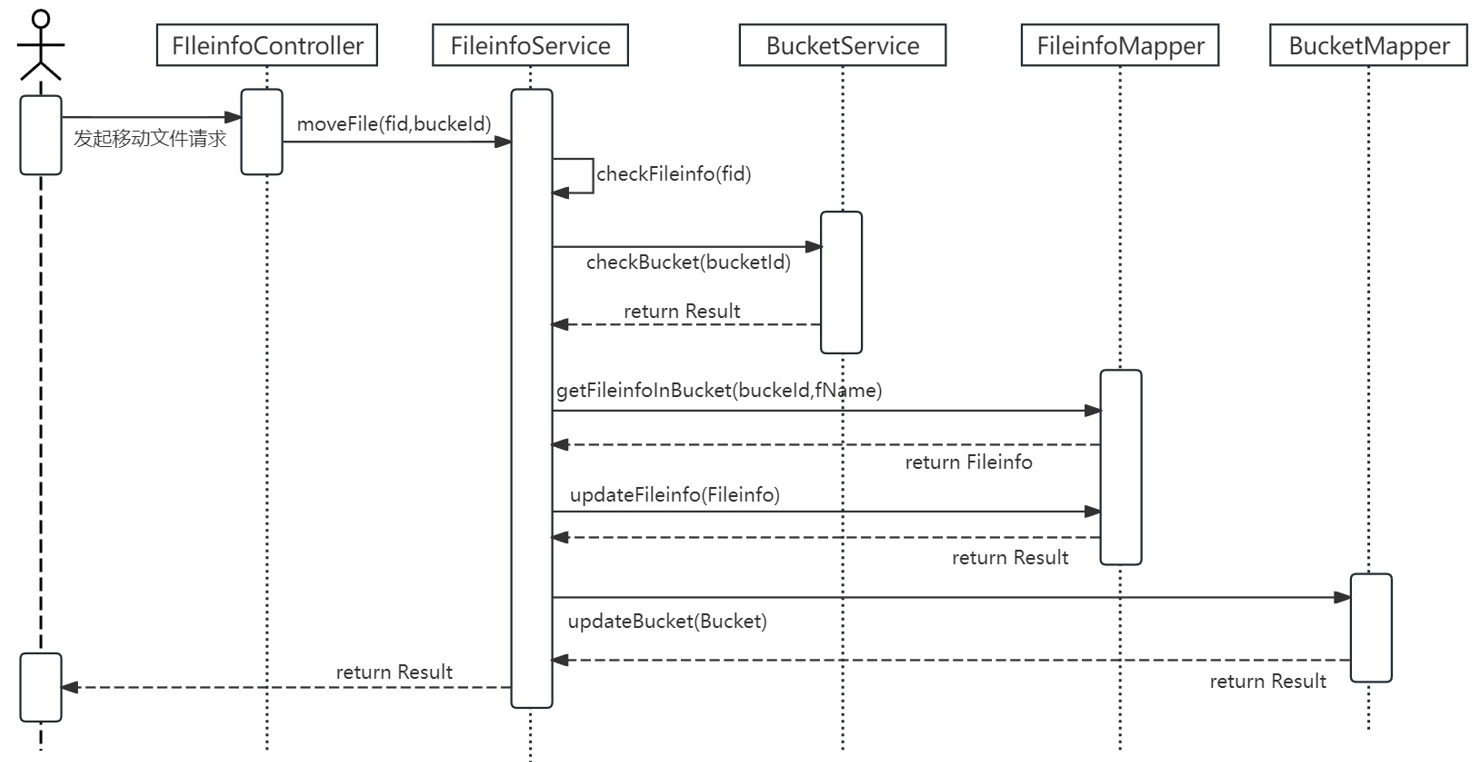
\includegraphics[width=0.96\textwidth]{移动文件时序图.png}
  \caption{移动文件时序图}
  \label{移动文件时序图}
\end{figure}

查看文件信息操作较为简单,在验证完文件的合法性后,只需用getFileinfoById将文件信息从元数据数据库中获取并返回即可。如果需要查看桶内的全部文件,则需要用checkBucket检测桶的合法性,然后调用getFileinfosByBucketId将数据返回即可。

\subsection{文件交互模块实现}
文件交互模块向用户提供文件上传、文件下载和文件删除这三个功能。这个模块的类图如图\ref{文件交互模块类图}所示。

\begin{figure}
  \centering
  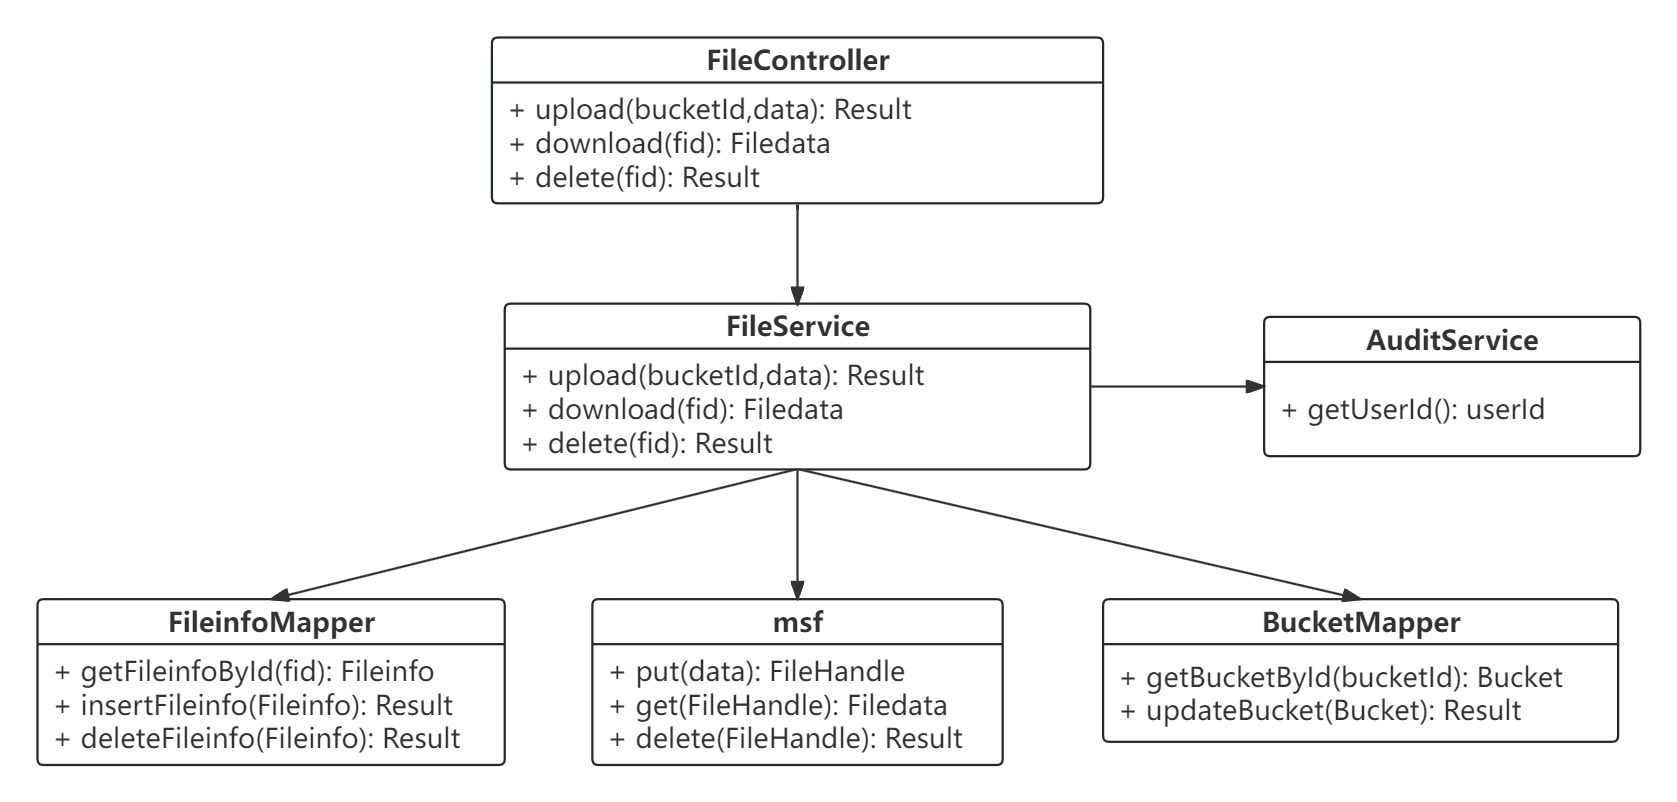
\includegraphics[width=1\textwidth]{文件交互类图.jpg}
  \caption{文件交互模块类图}
  \label{文件交互模块类图}
\end{figure}

文件交互模块中的FileController负责接收请求,接收请求后转交给FileService,FileService通过调用msf来和对象数据存储模块进行交互,msf是对象存储模块对外暴露的接口,向功能模块提供了三个方法来帮助功能模块完成文件的交互,FileinfoMapper和BucketMapper用来处理文件的元数据。

\begin{figure}
  \centering
  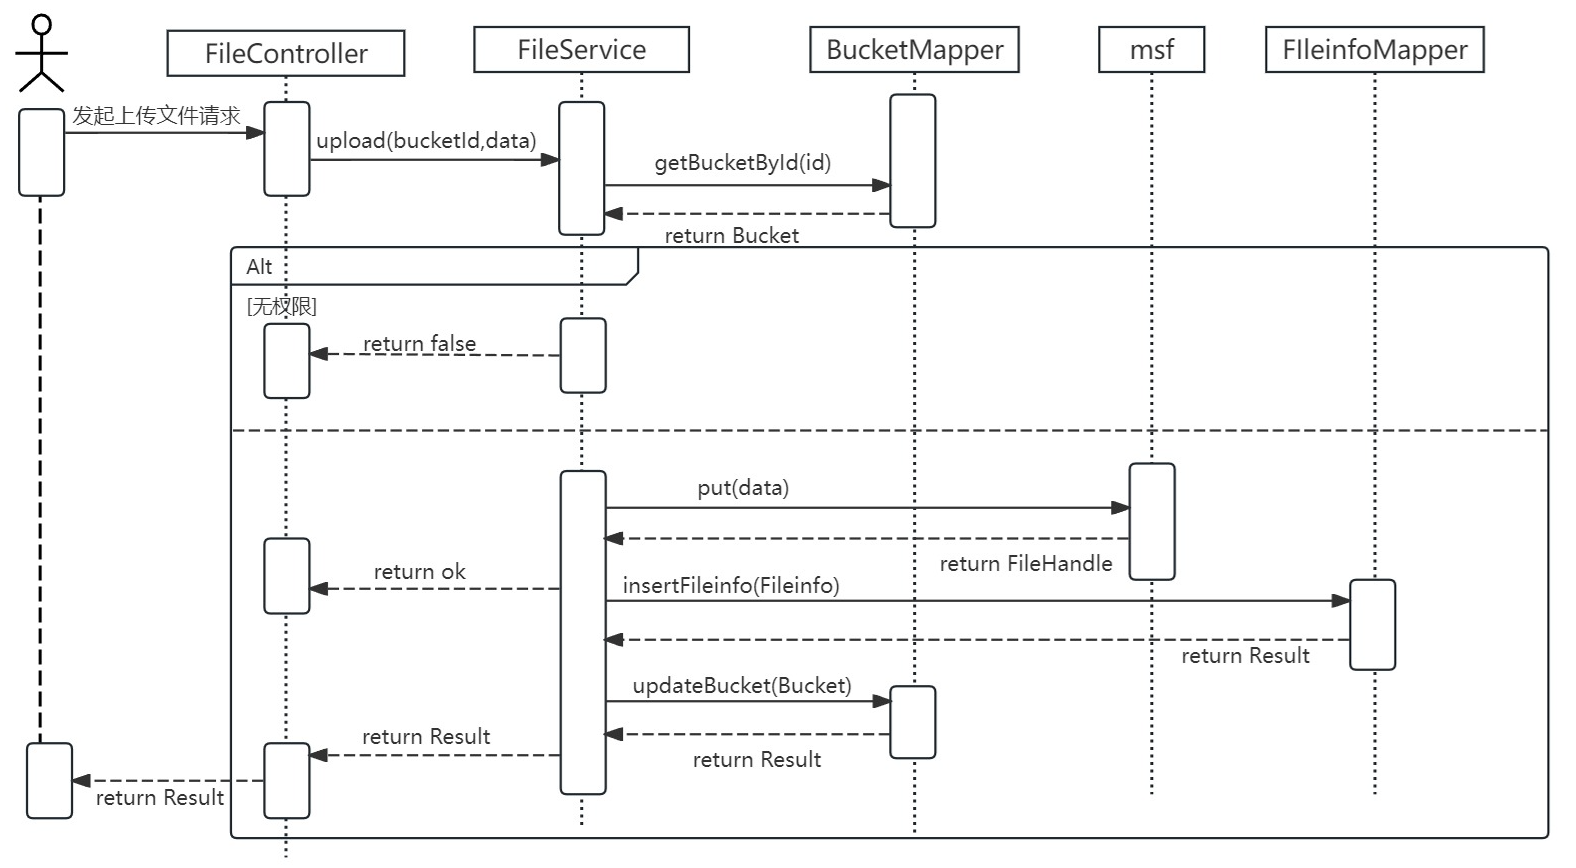
\includegraphics[width=1\textwidth]{上传文件时序图.png}
  \caption{文件上传时序图}
  \label{文件上传时序图}
\end{figure}

文件上传的时序图如图\ref{文件上传时序图}所示,FileService接收到请求后首先会调用getBucketById方法来获取桶的信息,然后检查用户是否有向这个桶上传文件的权限,如果没有上传的权限则会直接返回错误,如果有则调用msf的put方法将文件上传,得到这个文件的FileHandle后利用FileinfoMapper的insertFileinfo方法将文件的元数据写入元数据数据库中,最后还需要调用updateBucket来更新桶的相关信息。

文件下载操作完整工作情况时的时序图如图\ref{文件下载时序图}所示。FileService接收到请求后首先会调用getFileinfoById方法来获取文件的信息,如果不存在该文件则返回错误,如果文件存在还要验证用户是否有下载权限,这一步需要利用getBucketById来找到文件所属的桶。权限检测完毕后用msf中的get方法来下载文件数据并返回。

\begin{figure}
  \centering
  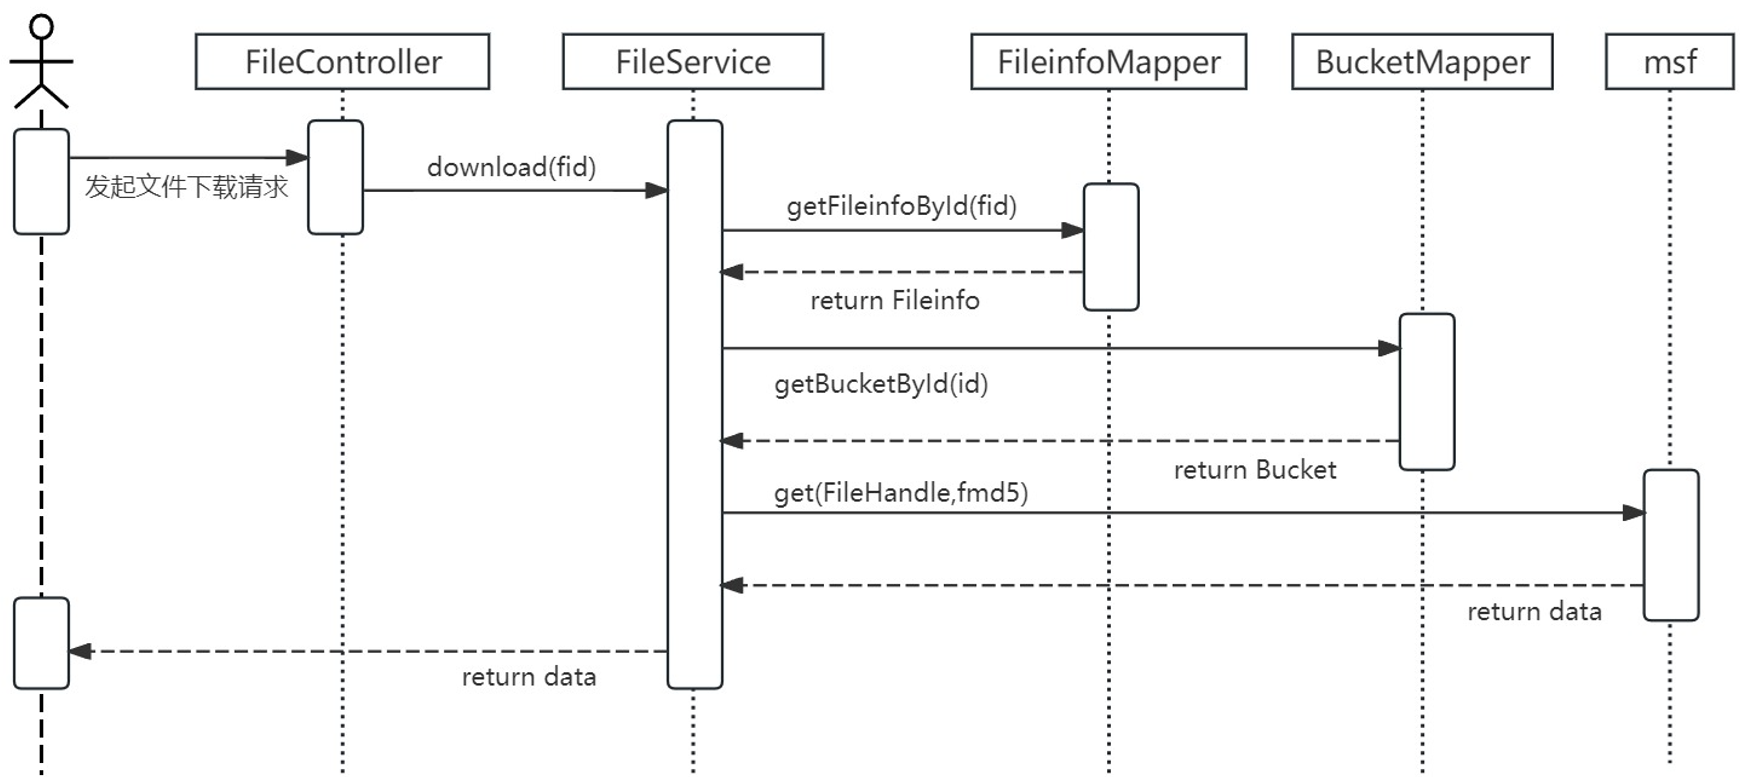
\includegraphics[width=0.9\textwidth]{文件下载时序图.png}
  \caption{文件下载时序图}
  \label{文件下载时序图}
\end{figure}

文件删除操作完整工作情况时的时序图如图\ref{删除文件时序图}所示。和文件下载一样,FileService接收到请求后先调用getFileinfoById方法来获取文件的信息,如果文件不存在或不属于自己则返回错误,反之则用FileinfoMapper的deleteFileinfo方法和BucketMapper方法updateBucket删除相关元数据,再利用msf的delete方法将文件删除。

\begin{figure}
  \centering
  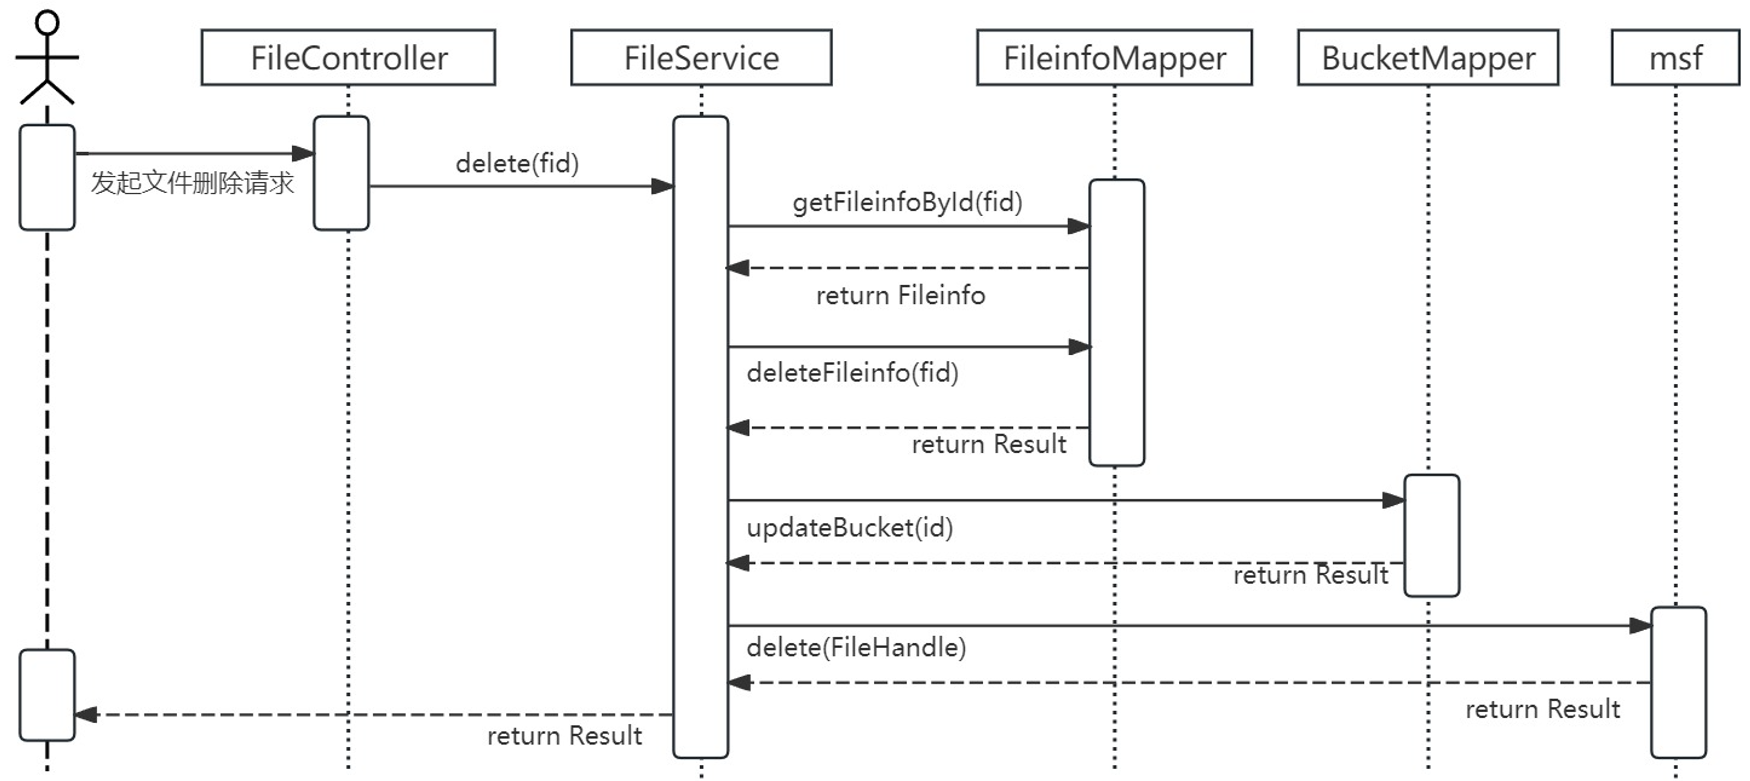
\includegraphics[width=1\textwidth]{文件删除时序图.png}
  \caption{删除文件时序图}
  \label{删除文件时序图}
\end{figure}

\section{本章小结}%5.4
本章的主要工作是在第四章的概要设计的基础上,详细地阐述了该应用的具体实现细节,首先介绍系统中对象数据存储模块的实现细节,包括master、storage、worker和msf这四部分内容,这个模块是系统的核心,负责对象数据的落地存储。然后介绍了功能模块的具体细节,包括用户数据管理模块、桶数据管理模块、文件管理模块和文件交互模块这四个功能模块,这四个模块负责实现系统的功能,它们通过和对象数据存储模块和元数据模块进行交互来完为用户提供所需的数据。

至此,我们完成了该分布式对象存储系统的实现,在本章基础上,下一章节,我们将完成对系统的测试。 
